%
% this file is encoded in utf-8
% v2.0 (Apr. 5, 2009)

\documentclass[12pt, a4paper]{ntuthesis}

% 除非校方修改了論文格式 (margins, header, footer, 浮水印, 中文數字之章別)
% 或者需要增加所用的 LaTeX 套件,
% 或者要改預設中文字型、編碼
% 否則毋須修改本檔內容
% 論文撰寫,請修改以 my_  開頭檔名的各檔案

\usepackage{CJKutf8}  %%% ZZZ %%% macro for Chinese/Japanese/Korean processing
\usepackage{CJKnumb} %%% ZZZ %%% for Chinese numbering capability
\usepackage[nospace]{cite}  % for smart citation
%\usepackage{geometry}  % for easy margin settings
\usepackage{ntuthesis}
\usepackage{multirow,multicol,rotating}

%
% margins setting
%\geometry{verbose,a4paper,tmargin=3.5cm,bmargin=2cm,lmargin=4cm,rmargin=2cm}
%

% 插圖套件 graphicx
% 使用者工作流程是用 pdftex 還是 latex + dvipdfmx?
% 視情況而有不同的參數
% 這裡作自動判斷
% 參考自
% http://www.tex.ac.uk/cgi-bin/texfaq2html?label=ifpdf
\newcommand\mydvipdfmxflow{dvipdfmx}
\newcommand\mypdftexflow{pdftex}
\ifx\pdfoutput\undefined
  % not running pdftex
  \usepackage[dvipdfm]{graphicx}
  \newcommand\myworkflow{dvipdfmx}  % set the flag for hyperref
\else
  \ifx\pdfoutput\relax
    % not running pdftex
    \usepackage[dvipdfm]{graphicx}
    \newcommand\myworkflow{dvipdfmx}  % set the flag
  \else
    % running pdftex, with...
    \ifnum\pdfoutput>0
      % ... PDF output
      %\usepackage[pdftex]{graphicx}
      \newcommand\myworkflow{pdftex}  % set the flag
    \else
      %...DVI output
      \usepackage[dvipdfm]{graphicx}
      \newcommand\myworkflow{dvipdfmx}  % set the flag
    \fi
  \fi
\fi

% 增強功能型頁楣 / 頁腳套件
\usepackage{fancyhdr}  % 借用此套件來擺放浮水印 
% (佔用了 central header)
% 不需要浮水印的使用者仍可利用此套件,產生所需的 header, footer
%
% 啟動 fancy header/footer 套件
\pagestyle{fancy}
\fancyhead{}  % reset left, central, right header to empty
\fancyfoot[C]{\thepage} %中間 footer 擺放頁碼
\renewcommand{\headrulewidth}{0pt} % header 的直線; 0pt 則無線

% 如果不需要任何浮水印,則請把下列介於 >>> 與 <<< 之間
% 的文字行關掉 (行首加上百分號)
%% 浮水印 >>> 
%\input{yzu_watermark.tex}
%% <<< 浮水印

% 如需額外的頁楣 (header) 或 footer,請在 my_headerfooter.tex 裡依例修改
% 它的預設內容是都關掉,可依需要打開
%
% this file is encoded in utf-8
% v2.0 (Apr. 5, 2009)

%%%%%%% 其他的 header (left, right) 定義
% 底下定義了一些常見的 header 型式
% 預設情況是關掉的
% 使用者可以視需要將之打開
% 也就是把下列介於 >>> 與 <<< 之間
% 的文字行打開 (行首去掉百分號)

%% header >>>
%\renewcommand{\chaptermark}[1]{%
%\markboth{\prechaptername\ \thechapter\ \postchaptername%
%\ #1}{}%
%}  %定義 header 使用的「章」層級的戳記
%\fancyhead[L]{} % 左 header 為空
%\fancyhead[R]{\leftmark}  % 右 header 擺放「章」層級的戳記 (以 \leftmark 叫出)
%\renewcommand{\headrulewidth}{0.4pt}  % header 的直線 0.4pt; 0pt 則無線
%% <<< header

%%%%%%% 其他的 footer (left, right) 定義
% 底下定義了一些常見的 footer 型式
% 預設情況是關掉的
% 使用者可以視需要將之打開
% 也就是把下列介於 >>> 與 <<< 之間
% 的文字行打開 (行首去掉百分號)

%% footer >>>
%\fancyfoot[L]{} % 左 footer 為空
%\fancyfoot[R]{\small{YZU \LaTeX\ v2.0}} % 右 footer 擺放論文格式版本
%\renewcommand{\footrulewidth}{0.4 pt} % footer 的直線 0.4pt; 0pt 則無線
%% <<< footer




%%%%%%%%%%%%%%%%%%%%%%%%%%%%%%
%%%% 非必要的套件,但很實用
\usepackage{amsmath} % 各式 AMS 數學功能
\usepackage{amssymb} % 各式 AMS 數學符號
\usepackage{mathrsfs} %草寫體數學符號,在數學模式裡用 \mathscr{E} 得草寫 E
\usepackage{listings} % 程式列表套件
\usepackage{subfig}
\usepackage{tabularx}
\usepackage{url}
\usepackage[usenames,dvipsnames]{xcolor}
\usepackage{pgf}
\usepackage{tikz}
\usetikzlibrary{arrows,automata,positioning}



% Title Page
\renewcommand{\enTitle}{Enhanced Semantic Retrieval of Spoken Content with Query Expansion and Automatically Discovered Acoustic Patterns}  %英文標題
\renewcommand{\zhTitle}{使用查詢詞擴展與自動習得之聲學組型強化語音數位內容之語意檢索}  %中文標題
\renewcommand{\authorZhName}{李昀樵}  %作者中文姓名
\renewcommand{\authorEnName}{Yun-Chiao Li}  %作者英文姓名
\renewcommand{\authorStudentID}{R01942062}  %作者學號
\renewcommand{\advisorZhName}{李琳山}  %指導教授中文姓名
\renewcommand{\advisorEnName}{Lin-Shan Lee}  %指導教授英文姓名
\renewcommand{\zhCollegeName}{電機資訊學院}  %學院中文名稱
\renewcommand{\enCollegeName}{College of Electrical Enginnering and Computer Science}  %學院英文名稱
\renewcommand{\zhDepartmentName}{電信工程學研究所}  %系所中文名稱
\renewcommand{\enDepartmentName}{Graduate Institute of Communication Engineering}  %系所英文名稱
\renewcommand{\rocYear}{一百零三}  %中華民國紀年年份
\renewcommand{\zhMonth}{六}  %中文月份
\renewcommand{\enYear}{2014}  %公元紀年
\renewcommand{\enMonth}{June}  %英文月份
\renewcommand{\oralDate}{103 年 6 月 23 日}  %口試日期

%
% listing setting
\lstset{breaklines=true,% 過長的程式行可斷行
extendedchars=false,% 中文處理不需要 extendedchars
texcl=true,% 中文註解需要有 TeX 處理過的 comment line, 所以設成 true
comment=[l]\%\%,% 以雙「百分號」做為程式中文註解的起頭標記,配合 MATLAB
basicstyle=\small,% 小號字體, 約 10 pt 大小
commentstyle=\upshape,% 預設是斜體字,會影響註解裏的英文,改用正體
%language=Octave % 會將一些 octave 指令以粗體顯示
}

\usepackage{url} % 在文稿中引用網址,可以用 \url{http://www.yzu.edu.tw} 方式

%%%% 以上為非必要套件
%%%%%%%%%%%%%%%%%%%%%%%%%%%%%%

%%% 以下是 hyperref 套件
%%%%%%%%%%%%%%%%%%%%%%%%%%%%%%
% hyperref 會擾亂 cite.sty 對文獻號碼縮編的排版,所以依據
% http://www.ctan.org/tex-archive/macros/latex/contrib/hyperref/
% 作如下的更動,使得 hyperref 不做文獻號碼的超連結。
\makeatletter
\def\NAT@parse{\typeout{This is a fake Natbib command to fool Hyperref.}}
\makeatother

% hyperlinkable table of contents
% 章節目錄、圖表超連結
\ifx\myworkflow\mydvipdfmxflow
	\usepackage[dvipdfmx, debug, colorlinks, linkcolor=black, citecolor=black, urlcolor=black, unicode]{hyperref}
\else
	\usepackage[pdftex, debug, colorlinks, linkcolor=black, citecolor=black, urlcolor=black, unicode]{hyperref}	
\fi

% if hyperref is not used (e.g., in LyX application)
% define dummy \phantomsection for those occurences
%   in yzu_frontpages.tex, yzu_backpages.tex, my_appendix.tex
\ifx\hypersetup\undefined
	\newcommand\phantomsection{}
\fi

% hyperref跟algorithm衝突,hyperref必須放在algorithm前面
\usepackage{algorithm}
\usepackage{algorithmic}
%%%% 以上為所有套件
%%%% 
%%%% 

% global page layout
%\newcommand{\mybaselinestretch}{1.5}  %行距 1.5 倍 + 20%, (約為 double space)
%\renewcommand{\baselinestretch}{\mybaselinestretch}  % 論文行距預設值
%\parskip=2ex  % 段落之間的間隔為兩個 x 的高度
%\parindent = 0Pt  % 段首內縮由 CJK 控制,所以這裡就設成不內縮

%%%%%%%%%%%%%%%%%%%%%%%%%%%%%
%  end of preamble
%%%%%%%%%%%%%%%%%%%%%%%%%%%%%
%
\begin{document}
\begin{CJK}{UTF8}{bsmi}   %%% ZZZ %%%  <<< 在這裡更改預設中文字型、編碼
% 編碼:UTF8, Bg5, ...
% 中文字型名稱:TeXLive 安裝有一套明體字 bsmi, 楷書與其他字型視你的 LaTeX CJK 系統裝設情況而定

% 針對 latex + dvipdfmx 工作流程在 hyperref 套件的影響下,圖檔的辨識力退化
% 所作的權宜措施。可能是因為 TeXLive2007 hyperref 裏的
% 客製 graphicx / dvipdfmx 的設定檔不夠新
\ifx\myworkflow\mydvipdfmxflow
	\DeclareGraphicsExtensions{.pdf,.png,.jpg,.eps}
	\DeclareGraphicsRule{.pdf}{eps}{.bb}{}
	\DeclareGraphicsRule{.png}{eps}{.bb}{}
	\DeclareGraphicsRule{.jpg}{eps}{.bb}{}
\fi

% global CJK setting
\CJKindent  %%% ZZZ %%%  段首內縮兩格

% 載入中文名詞的定義:例如,Figure -->「圖」, Chapter -->「第 x 章」
%
% this file is encoded in utf-8
% v2.0 (Apr. 5, 2009)

% 下列中文名詞的定義,如果以註解方式關閉取消,
% 則會以系統原先的預設值 (英文) 替代
% 名詞 \prechaptername 預設值為 Chapter
% 名詞 \postchaptername 預設值為空字串
% 名詞 \tablename 預設值為 Table
% 名詞 \figurename 預設值為 Figure
\renewcommand\prechaptername{第} % 出現在每一章的開頭的「第 x 章」
\renewcommand\postchaptername{章}
\renewcommand{\tablename}{表} % 在文章中 table caption 會以「表 x」表示
\renewcommand{\figurename}{圖} % 在文章中 figure caption 會以「圖 x」表示

% 下列中文名詞的定義,用於論文固定的各部分之命名 (出現於目錄與該頁標題)
\newcommand{\nameInnerCover}{書名頁}
\newcommand{\nameCommitteeForm}{論文口試委員審定書}
\newcommand{\nameCopyrightForm}{授權書}
\newcommand{\nameCabstract}{中文摘要}
\newcommand{\nameEabstract}{英文摘要}
\newcommand{\nameAckn}{誌謝}
\newcommand{\nameToc}{目錄}
\newcommand{\nameLot}{表目錄}
\newcommand{\nameTof}{圖目錄}
\newcommand{\nameSlist}{符號說明}
\newcommand{\nameRef}{參考文獻}
\newcommand{\nameVita}{自傳}



% 如果不需要以中文數字一、二、三呈現章別,例如「第一章」
% 則請把下列介於 >>> 與 <<< 之間
% 的文字行關掉 (行首加上百分號), 會以「第 1 章」呈現
%% 中文數字章別 >>>
%
% this file is encoded in utf-8
% v2.0 (Apr. 5, 2009)

% 請依需要選擇其中一種表現方式,把它所對應的指令列打開,其他沒有用到的表現方式的對應指令列請關閉。(用行首百分號)

%% 第一種目錄格式:
%%	1  簡介 ............................ 1
%%
%%      章別 (chapter counter) 「1」前後沒有其他文字,
%%
%%      內文章標題是
%%		第 1 章	簡介
%%	\tocprechaptername, \tocpostchaptername 都設成沒有內容的空字串
%%	\tocChNumberWidth 設成 1.4em (預設)
%%      底下三行指令請打開
%\renewcommand\tocprechaptername{}
%\renewcommand\tocpostchaptername{}
%\setlength{\tocChNumberWidth}{1.4em}


%% 第二種目錄格式:
%%	一、簡介 ............................ 1
%%
%%      章別 (chapter counter) 「一」前沒有文字,後有頓號,
%%
%%      內文章標題是
%%		第一章		簡介
%%	\tocprechaptername 設成沒有內容的空字串
%%	\tocpostchaptername 設成頓號
%%	\tocChNumberWidth 設成 2em
%%      底下四行指令請打開 (預設)
\renewcommand\countermapping[1]{\CJKnumber{#1}}
\renewcommand\tocprechaptername{}
\renewcommand\tocpostchaptername{、}
\setlength{\tocChNumberWidth}{2em}


%% 第三種目錄格式:
%%	第一章、簡介 ......................... 1
%%
%%      章別 (chapter counter) 「一」前有「第」,後有「章」與頓號,
%%      內文章標題是
%%		第一章		簡介
%%	\tocprechaptername 設成「第」
%%	\tocpostchaptername 設成「章、」
%%	\tocChNumberWidth 設成 3em
%%      底下四行指令請打開
%\renewcommand\countermapping[1]{\CJKnumber{#1}}
%\renewcommand\tocprechaptername{第}
%\renewcommand\tocpostchaptername{章、}
%\setlength{\tocChNumberWidth}{3em}



%% 可以依照需要作彈性的設定
%%
%% 章別 (數字,包括後面的字串) 的寬度 \tocChNumberWidth,
%% 會影響章名與章別之間的間隔 (太少則相疊,太多則留白)
%% 建議設成 \tocpostchaptername 內容字數加一,做為 em 的倍數,
%% 但至少也要有 1.4 倍。

%% <<< 中文數字章別

%%% 以下是載入前頁、本文、後頁
% 請勿更動
% 如需針對個別章節獨立編譯
% 請在 my_chapters.tex 檔裡對個別章節的 \input 指令以行首百分號方式做開關。

\NTUtitlepage  % 產生論文封面

\newpage
\setcounter{page}{1}
\pagenumbering{roman}

\NTUoralpage  % 產生口試委員會審定書

\mydoublespacing
%\begin{acknowledgement} %誌謝
   %請在這裡寫您的誌謝辭 
%\end{acknowledgement}

\begin{zhAbstract}  %中文摘要
  % 語音辨識(Speech Recognition)問題可視為針對一段語音訊號求出所對應的詞串。
  % 這個問題由於結構十分複雜,
  % 所以在傳統上,
  % 我們都是將問題用貝氏定理(Bayes Theorem)拆解成聲學模型(Acoustic Model)與語言模型(Language Model)兩個子問題,
  % 這兩個子問題結構比較單純,
  % 方便我們用隱藏式馬可夫模型(Hidden Markov Model)來解決。

  % 但隱藏式馬可夫模型估測參數的時候傳統上使用最大相似度估測法(Maximum Likelihood Estimation),
  % 容易在不同模型之間造成混淆。
  % 乃有人提出鑑別式訓練法(Discriminative Training),
  % 讓傳統的模型架構也具備鑑別力。

  % 隨著機器學習領域的發展,
  % 我們逐漸有能力直接解決語音辨識的問題而未必需要將它拆成兩個子問題,
  % 而這樣的模型多半天生就具備鑑別能力。
  % 本論文便嘗試在這樣的架構下先進行初步的音素辨識。
  % 論文中使用的模型為結構化支持向量機(Structural Support Vector Machine)。
  % 實驗顯示,
  % 所獲得之音素正確率(Phone Accuracy)會超過串接式系統(Tandem System)的1\%。

\end{zhAbstract}

{
%\zhKaiFont
\mysinglespacing\selectfont
\tableofcontents %目錄

\listoffigures  %圖目錄

\listoftables  %表目錄
\par
}

\newpage
\setcounter{page}{1}
\pagenumbering{arabic}


\chapter{導論}
  \section{研究動機}
現在是一個資訊爆炸的時代,每天資訊的增長量是十分驚人的,因此,我們需要一套好的檢索系統 (Retrieval System) 幫助我們快速地瀏覽資訊,並找到其中有用的部分,在過去已有許多文字檢索系統與演算法被開發出來並應用於產業中,如 Google Search、Microsoft Bing Search、Yahoo
Search等。但近年來隨著科技與網際網路的興起,語音文件量正蓬勃地增加當中,隨著線上影片、會議錄音、線上課程等網站的興起,語音資料量越來越多,因此如何在其中找到使用者感興趣的資料便成為重要的議題,即為語音數位內容檢索 (Spoken Content Retrieval)~\cite{chelba2008retrieval, lee2005spoken}。相較於文字資訊檢索,語音資訊檢索面臨到更多的挑戰,如辨識錯誤、辨識訓練資料不足等問題,使得此問題更形困難。

近年來更由於智慧型手機的崛起與使用者需要在移動裝置上取得資訊的強烈需求,促使許多網路公司一一推出了自家的用語音輸入來檢索文字資訊的系統,如 Google 公司推出的語音檢索功能即可讓使用者在手機或瀏覽器的介面上以語音輸入,由 Google 將其辨識成文字後再於 Google 的搜尋引擎上檢索資訊。 Apple 公司推出的個人語音助理 Siri,也讓使用者能以十分自然的方式對 Siri 說出想要查詢的查詢詞 (Query) ,由 Siri 辨識後在網路上檢索,並將檢索結果分門別類整理好後呈現給使用者看。如上述所說的這類檢索系統是用語音輸入的查詢詞去檢索大量的文字資訊,此方法稱為人聲檢索 (Voice Search),和本論文所探討的語音數位內容檢索 (Spoken Content Retrieval) 完全不同。

本論文所探討的語音數位內容檢索,是指由於網路上有大量的多媒體文件,如線上影片、會議錄音、線上課程、電視連續劇、演講等,而使用者也有搜尋這些多媒體文件的需求,此類允許使用者用文字或聲音輸入查詢詞並搜尋語音數位內容 (Spoken Content) 的系統稱為語音數位內容檢索 (Spoken Content Retrieval),如 TED (美國著名的演講網站) 會將網站上的演講內容轉寫 (Transcript) 成為文字,並允許使用者於網站上輸入文字檢索這些影片的文字稿。 Youtube 也會於離線時將其網站上的影片辨識成文字,但目前尚不支援直接輸入查詢詞檢索影片轉寫的方式,可以期待未來 Youtube 會開放這方面的功能。只是上述兩個例子仍要倚賴人工的轉寫,要完全只靠機器自動辨識仍不容易做到。這種語音數位內容檢索將是本論文主要的研究主軸。

由於以上所述的語音數位內容檢索系統大部分都是回傳給使用者有出現查詢詞的語音文件,但如此一來使用者必須完美地輸入有出現在語音文件中的查詢詞,如果使用者心中想的概念與語音文件中的詞彙不匹配,則檢索系統的成效就會大大地降低。使用者通常期待的是系統會查到所有與查詢詞「語意上相關」的文件,比如查詢詞為「東京旅遊」的話,使用者想要查詢到的文件通常包含與「東京住宿」、「東京景點」等有關的結果,而不只是那些包含了「東京旅遊」的文件。此即為語意檢索 (Semantic Retrieval) 的系統。語意檢索一個很常見的實作方法是查詢詞擴展 (Query
Expansion),查詢詞擴展的精神是先進行第一次檢索,得到第一次檢索結果 (First-pass Retrieval Result),並從其中最相關的前幾篇中找出常常出現卻不是在所有文章中都常常出現的詞,再加入到原查詢詞中成為擴展後查詢詞 (Expanded Query),再使用擴展後查詢詞進行第二次檢索 (Second-pass Retrieval)。

本論文想要探討的主題將是針對語音數位內容之語意檢索 (Semantic Retrieval of Spoken Content),是指系統在接受到口語形式或文字形式的查詢詞之後,儘可能回傳給使用者所有與查詢詞語意上相關的語音文件。由於傳統的語音數位內容之語意檢索系統主要的實作方法為先將語音文件辨識為文字檔後,對文字做檢索,但在辨識之中,會遇到如詞典外詞彙
(OOV)、辨識錯誤等情況,更甚者,許多語音中珍貴的資訊如韻律 (Prosody)、語速 (Speaking Rate)和語者特徵 (Speaker Characteristic)等在辨識後就消失了,十分地可惜。因此本論文試圖結合一套自動習得的聲學組型 (Automatically Discovered Acoustic Patterns) 至語音數位內容之語意檢索當中,以期改善傳統的檢索系統。

\section{研究方向}
本論文之研究方向為使用自動習得之聲學組型強化語音數位內容之語意檢索,主要包含以下幾點:

\begin{itemize}
\itemsep -2pt %reduce space between items
  \item  傳統的語意檢索系統是先將語音文件辨識為文字後,將輸入的文字查詢詞進行查詢詞擴展 (Query Expansion),再用擴展後查詢詞對辨識後的文字進行檢索,但如此一來許多語音訊號中的珍貴的聲學資訊就消失了。因此本章中在文字的查詢詞擴展之外,再加入一套自動習得之聲學組型的查詢詞擴展,並結合兩套查詢詞擴展之結果回傳給使用者。

  \item  更進一步地,本論文希望能處理口語形式的查詢詞,可以用口語形式的查詢詞進行語音數位內容之語意檢索。另一方面,語意檢索通常需要自動語音辨識系統 (Automatically Speech Recognition) 將聲音辨識成文字,進而得到語意上的資訊,但自動語音辨識系統的訓練是很昂貴的,需要大量標注完善的語料才能訓練出很好的聲學與語言模型。因此本章中會將聲音辨識成聲學組型,並在聲學組型上進行查詢詞擴展,進而達到非監督式語音數位內容之語意檢索 (Unsupervised Semantic Retrieval of Spoken Content)。
  
  \item  由於聲學組型在訓練時是盡量將聲音很像之片段盡量分群 (Clustering) 在一起,但如此一來會使得同一個聲學組型中包含了大量同音但對應到不同字詞的聲學組型,會使得檢索系統的成效大幅下降。因此本章使用基於遞迴式類神經網路語言模型 (Recurrent Neural Network Language Model, RNNLM) 之詞表示法 (Word Representation) 將這些聲學組型按照句法 (Syntactics) 和語意 (Semantics) 進一步分群為不同的聲學組型,進而提升檢索系統之成效。
   
  \item  最後,由於近年來行動裝置與穿戴式裝置日漸流行,使用者也漸漸習慣於在行動裝置上用語音輸入並取得資訊,因此本論文基於 Google 眼鏡 ( Google Glass) 上推出了一套語音翻譯系統與語音數位內容檢索系統,讓使用者能夠隨時隨地用最方便的方法取得新資訊。

\end{itemize}

\section{章節安排}
本論文之章節安排如下:

\begin{itemize}
\itemsep -2pt %reduce space between items
  \item  第二章:介紹本論文相關背景知識。
  \item  第三章:介紹如何以聲學組型改善監督式語意檢索。
  \item  第四章:介紹如何以聲學組型實現非監督式語意檢索。
  \item  第五章:介紹如何以遞迴式類神經網路語言模型產生之詞向量改善第四章的非監督式語音文件檢索。
  \item  第六章:介紹如何將本論文之語音檢索系統與語音翻譯系統實作到 Google Glass 上。
  \item  第七章:本論文之結論與未來研究方向。
\end{itemize}


\chapter{背景知識}
  \section{資訊檢索}
資訊檢索的目的是幫助使用者迅速地在資料庫中找尋所需要的文件。典型的資料檢索系統流程如圖~\ref{fig:chap2_retrieval}:首先,當使用想要找尋與某個主題(Topic)或概念(Concept)相關的文件時,使用者會先在腦中將所想的概念轉化成查詢詞,這裡的查詢詞長度不一,可以像一個句子、數個詞、單詞、或是字均可。根據系統設計的不同,查詢詞也可以是圖、照片、聲音、影片等皆可。
\begin{figure}
\centering
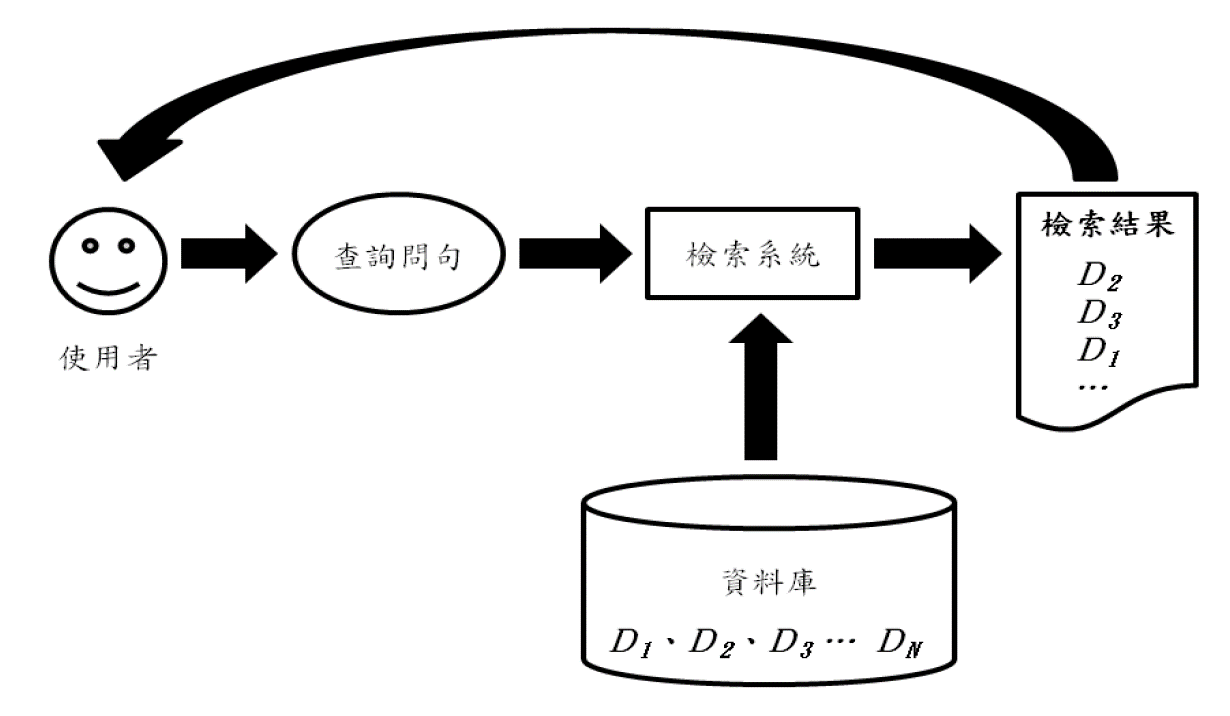
\includegraphics[scale=0.5]{images/chap2_retrieval.png}
\caption{資訊檢索的基本架構} \label{fig:chap2_retrieval}
\end{figure}

在得到查詢詞之後,系統會依照查詢詞$Q$與資料庫中的文件$D$計算相關分數$S(Q, D)$,一個系統的好壞通常決定於計算的相關分數是否準確。相關分數可以如下計算:

\[
S(Q, D) = P(r|Q, D)
\]

此處的$P(r|Q, D)$是代表當給定查詢詞$Q$和文件$D$時,兩者相關的機率有多少,這種排序方法稱為機率排序原則(Probability Ranking Principle, PRP)~\cite{amati2002probabilistic},而用來計算$P(r|Q, D)$的方法則有很多種,包括布林模型(Boolean Model)、向量空間模型(Vector Space Model)、機率模型(Probabilistic Model)~\cite{robertson1977probability}等。本論文使用的方法是基於語言模型的檢索(Language Model Based Retrieval)~\cite{chia2010statistical},先把查詢詞$Q$和文件$D$表示成兩個語言模型後,再計算兩個語言模型的KL散度 (Kullback–Leibler Divergence) 作為兩者的距離,具體作法見~\ref{subsec:retrievalsystem}節。
	
\subsection{口述語彙偵測與語意檢索}
語音檢索大致可分為兩大領域:口述語彙偵測 (Spoken Term Detection)~\cite{hazen2009query} 與語意檢索 (Semantic Retrieval)~\cite{lee2012improved} 。口述語彙偵測的目的是在所有語音文件集合中,找到包含語音查詢詞 (Spoken Query) $Q$ 的所有語音文件,語意檢索的目的是在所有語音文件集合中,找到語意上與語音查詢詞 $Q$ 相關 (Semantically Relevant)
的所有語音文件。舉例來說,如果使用者對系統說了:「美國總統」一詞,一個好的口述語彙偵測系統應該要能回傳所有包含「美國總統」一詞的語音文件,但一個好的語意檢索系統應該要能回傳所有包含「白宮」、「歐巴馬」等使用者覺得與查詢詞相關的詞的文件。由於語意檢索系統必須自動地猜測使用者可能想要找的詞彙,並主動尋找,因此存在有許多的挑戰,語意檢索將是此篇論文主要的研究主題。

\section{傳統語音資訊檢索}
語音資訊檢索系統大致上可以視為由兩個部分組成:語音辨識系統與資訊檢索系統。語音辨識系統需要有事先訓練好的聲學模型和語言模型,系統再從語音文件中抽出聲學特徵,系統再把聲學特徵辨識成為文字轉寫。有了文字轉寫之後檢索系統會計算查詢詞和各文件轉寫的相關性,再把此相關分數排序後回傳給使用者。

\subsection{語音辨識系統}
語音系統的目的是將語音訊號準確地轉寫成文字。典型的語音辨識系統流程包含了抽取語音特徵、訓練聲學模型和語言模型、產生辨識結果。

\subsubsection{抽取聲學特徵}
通常需要先抽取聲學特徵,再將聲學特徵辨識成文字,而目前最廣為使用的聲學特徵為梅爾倒頻譜係數 (Mel-Frequency Cepstrum Coefficient, MFCC)~\cite{huang2001spoken}。

\begin{figure}
\centering
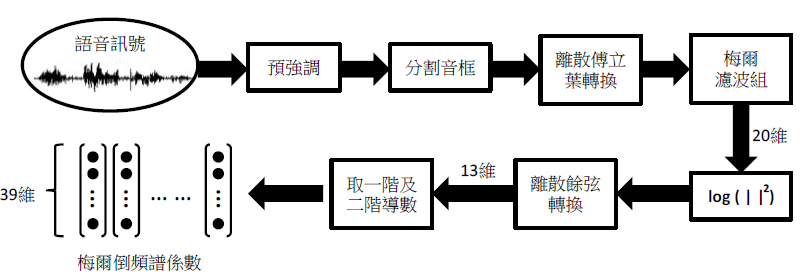
\includegraphics[scale=0.7]{images/chap2_mfcc.png}
\caption{梅爾倒頻譜係數抽取流程} \label{fig:chap2_mfcc}
\end{figure}

梅爾倒頻譜係數的抽取流程如圖~\ref{fig:chap2_mfcc}所示。第一步驟是預強調(Pre-emphasis)增加語音訊號裡高頻成分的比重。並且將語音訊號切成一連串長度固定且部分重疊的音框。再來,對每個音框內的訊號做離散傅立葉轉換,將每個音框內的訊號改為以頻率軸來表示。再把這些以頻率表示的訊號透過梅爾濾波組 (Mel-Filter Bank) 把每個音框壓縮成20維的向量。再把這些向量透過離散餘弦轉換 (Discrete Cosine Transform, DCT)
投射到彼此正交的軸上,此時可以忽略一些對訊號影響較小的維度,將訊號從20維降到12維,最後將音框中總體訊號能量相加後得到第13維。至此即可得到每個音框的13維向量,再對每個音框的13維向量取其一階與二階的時間軸導數 (Time Derivatives),即可形成39維的梅爾倒頻譜係數。

\subsubsection{訓練聲學模型}
\begin{figure}
\centering
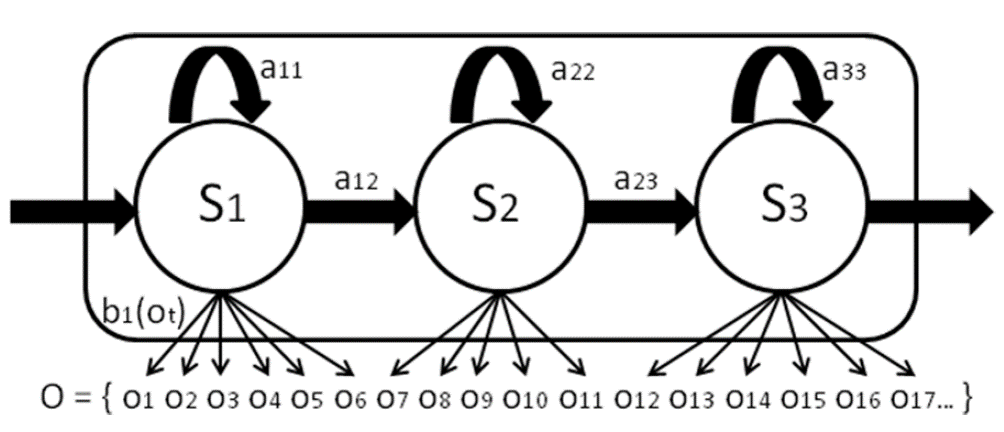
\includegraphics[scale=0.5]{images/chap2_hmm.png}
\caption{隱藏式馬可夫模型示意圖} \label{fig:chap2_hmm}
\end{figure}
訓練聲學模型最經典的方法即為隱藏式馬可夫模型 (Hidden Markov Models, HMM) ,其架構如圖~\ref{fig:chap2_hmm}  所示。隱藏式馬可夫模型是以一連串的狀態 (State) 模擬聲音隨時間轉換的特性。一個隱藏式馬可夫模型可以用來表示一個詞、字、音素、甚至是更小的聲學單位。而通常最常用的是三連音素是指每個狀態代表一個發音狀態。假設輸入的訊號為 $O = {o_t, t = 1, 2, 3, ...,
T}$,其中$O$代表一個語句,$o_t$為時間t的時候所對應到的聲學特徵,$T$則為語句的總長度。隱藏式馬可夫模型假設每個狀態之間有轉移機率 (Transition Probability),以$a_{ij}$表示從狀態$i$轉移到狀態$j$的機率:
    \begin{equation}
       a_{ij} = P(S_t = j | S_{t-1} = i)
    \end{equation}

$S_t$為$o_t$所屬的狀態,每一個狀態都是一個高斯混合模型 (Gaussian Mixture Model),用來表示在此狀態下聲學特徵的機率分布$b_j(o_t)$:
    \begin{equation}
    b_j(o_t) = P(o_t|S_t = j)
    \end{equation}
在此假設$o_t$只和當下的狀態$S_t$有關,而且狀態轉移只能停留在現在的狀態或是前往下一個狀態,無法後退或跳過一個狀態。

因此,一段聲音訊號$O$屬於某一段音素序列$w$的機率$P(O|w)$可表示為:
    \begin{equation}
    \begin{split}
       P(O|w) &= P(o_1o_2o_3...o_T | S_1S_2S_3...S_T) \\
              &= \Pi^T_{t=1}P(o_t|S_1S_2S_3...S_T) \\
              &= \Pi^T_{t=1}P(o_t|S_1S_2S_3...S_T) \\
              &= \Pi^T_{t=1}P(o_t|S_t, S_{t-1}) \\
              &= \Pi^T_{t=1}P(o_t|S_t)P(S_t|S_{t-1}) 
    \end{split}
    \end{equation}

    $w$是由一連串的狀態所構成,而$P(o_t|S_t)$可以用$b_j(o_t)$表示,$P(S_t|S_{t-1})$可以用$a_{ij}$來表示。這樣的聲學模型稱為隱藏馬可夫/高斯混合 (HMM/GMM) 模型。

\subsubsection{訓練語言模型}
語言模型是用來計算詞串$W$在某語言中出現的機率。假設$W = {w_1w_2...w_n}$,$w_i$代表在詞串$W$中出現的第$i$個詞彙,則$P(W)$可以表示成:
    \begin{equation}
        P(W) = P(w_1,w_2,w_3,...,w_n)
    \end{equation}
在此做個簡單的假設,詞彙$w_i$出現的機率會根據$w_i$前面的詞彙不同而有所差異。根據此假設將上式以條件機率展開則為:
    \begin{equation}
    P(W) = P(w_1, w_2, w_3,..., w_n) = \Pi^n_{k=1}P(w_k|w_1,w_2,...,w_{k-1}) 
    \end{equation}

    $w_1, w_2, ..., w_{k-1}$ 是$w_k$以前出現的詞彙,稱為歷史詞序列 (History Word Sequence),而$P(w_k| w_1, w_2, ..., w_{k-1})$則是$w_k$根據其歷史詞序列預測$w_k$出現的機率。

    如果歷史詞序列考慮的長度越長,所需的記憶體容量或硬體空間就越大,所以通常不會考慮很長的歷史詞序列。最常被使用的長度為詞雙連(Word Bigram)和詞三連(Word Trigram)的語言模型,分別對應到長度為2和3的歷史詞序列。因此詞雙連語言模型的機率可以近似為:
    \begin{equation}
    P(w_k|w_1, w_2, ..., w_{k-1}) \approx P(w_k|w_{k-1})
    \end{equation}

詞三連語言模型的機率可以近似為:
    \begin{equation}
    P(w_k|w_1, w_2, ..., w_{k-1}) \approx P(w_k|w_{k-2}, w_{k-1})
    \end{equation}

通常如果用來訓練語言模型的語料庫與要辨識的語句的領域越相近時,辨識結果會比較好,混淆度(Perplexity)也會越小。

\subsubsection{辨識結果}
把語音的訊號抽取出聲學特徵後,再經過聲學模型與語言模型計算出最佳的路徑後,即可得到此段語音的辨識結果,通常會將語音訊號辨識成兩種格式:詞圖(Lattice)~\cite{saraclar51lattice}和唯一最佳序列(One-Best
Transcription),詞圖像張網一樣,將每個時間所有可能的詞都呈現出來,而唯一最佳序列只呈現了詞圖上一條最可能的詞串當作辨識結果而已。通常在語音檢索時會使用詞圖來搜尋,因為語音辨識通常沒有辦法做到完全準確,可能會辨識成音很像的其他詞彙,比如「美國」可能會被辨識成「沒過」等等,如果使用唯一最佳序列的話,選中了正確的詞彙固然很好,但如果沒選中就會完全搜尋不出來了,而使用詞圖的話,這些可能的詞彙都會被表示在詞圖上,所以通常會使用詞圖來表示辨識的結果。

\begin{figure}
\centering
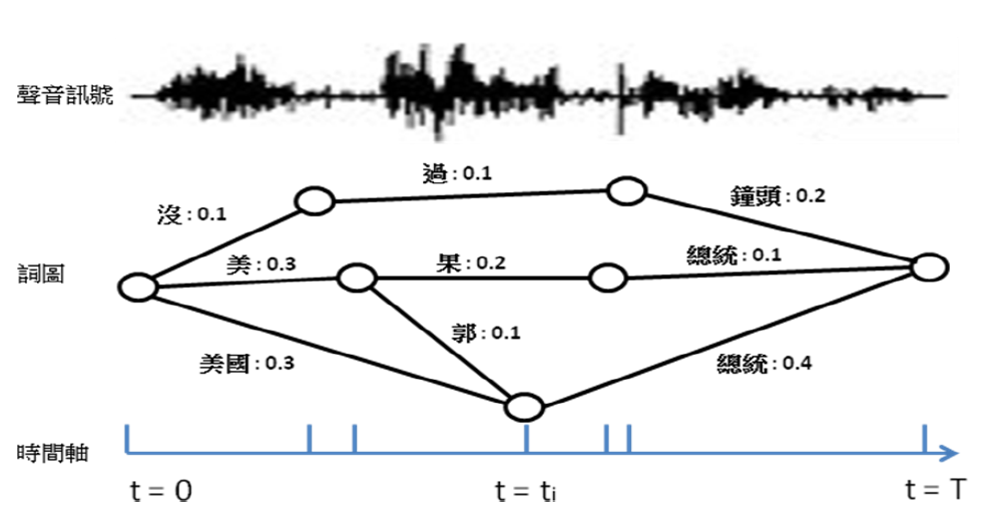
\includegraphics[scale=0.5]{images/chap2_lattice.png}
\caption{詞圖示意圖} \label{fig:chap2_lattice}
\end{figure}

如圖~\ref{fig:chap2_lattice}所示,詞圖主要由${N, A}$所構成,其中$N$是所有節點 (Node) 的集合,而$A$則是所有的詞弧 (Word Arc) 的集合。節點上存有各節點的時間資訊,而詞弧上除了有起始節點和終止節點外,還包含了在這個詞弧上的假定詞 (Word Hypothesis) 與此假定詞的信心分數 (Confidence Score) ,而此假定詞和信心分數都是由聲學模型和語言模型所計算出來的。

語音辨識系統的輸入是聲學特徵,並找出最有可能的詞彙串。因此相當於最大化以下的式子:
    \begin{equation}
    w^*_{seq} = argmax_{w_{seq} \in W_{seq}}P(w_{seq}|O)
    \end{equation}
O為輸入訊號之聲學特徵,$w_{seq}$為某個詞串,$W_{seq}$為所有$w_{seq}$之組合,$argmax$則是尋找一個$w_{seq}$使得$P(w_{seq}|O)$最大,此$w_{seq}$即為$w^*_{seq}$。但$P(w_{seq}|O)$無法直接被計算,所以根據貝氏定理 (Bayes' Theorem),可以表示如下:
    \begin{equation}
    P(w_{seq}|O) = \frac{P(O|w_{seq})P(w_{seq})}{P(O)}
    \end{equation}
由於$P(O)$是常數,可以不考慮,上式可簡化成:
    \begin{equation}
    P(w_{seq}|O) = P(O|w_{seq})P(w_{seq})
    \end{equation}

可以看得出來,$P(O|w_{seq})$可以由聲學模型求得,$P(w_{seq})$可以從語言模型中求得。求出來的$w^*_{seq}$即為唯一最佳序列。有時也會使用N最佳序列 (N-Best List) ,概念與唯一最佳序列很像,只是找出前N個讓$P(w_{seq}|O)$ 最大的$w_{seq}$。

\subsection{檢索系統}
\label{subsec:retrievalsystem}
檢索系統的目的主要是當使用者輸入查詢詞$Q$時,系統能夠計算出每個文件$X$與查詢詞間的相關分數$S(Q, X)$,進而將此相關分數排序後回傳給使用者。當系統接收到語音訊號時,系統會先對其抽取出聲學訊號,再經過聲學模型和語言模型辨識成唯一最佳序列或詞圖,一般來說,語音檢索系統使用詞圖的表現會比較好,所以以下主要就如何計算出查詢詞和詞圖的相關分數$S(Q, X)$加以介紹。

由於本章的檢索方式主要是基於語言模型的檢索 (Language model based retrieval)~\cite{zhai2008statistical, chia2010statistical},因此首先要把辨識所得的詞圖轉換為語言模型。對每個詞圖中的詞$t$,它在詞圖中的期望出現次數 (Expected Count) 可以如此計算:

\begin{equation}
E[t|x] = \sum_{\mu \in L(x)} N(t, \mu)P(\mu|x)
\end{equation}

$L(x)$是$x$的詞圖中所有的路徑,$\mu$是$L(x)$中的一條路徑,$N(t, \mu)$是$t$在$\mu$中出現的次數,$P(\mu|x)$是路徑$\mu$的事後機率(Posterior Probability)。

有了$E[t|x]$之後,就能把詞圖表示成單聯詞語言模型$\theta_x$:

\begin{equation}
P(t|\theta_x) = \frac{E[t|x]}{\sum_tE[t|x]}
\end{equation}

因為$\theta_x$裡沒有包含每個詞,為了讓$\theta_x$中每個詞都有一點機率,會再把$\theta_x$與一個背景語言模型 (Background Language Model) $\theta_b$做線性疊加,此過程稱為平滑化 (Smoothing)~\cite{zhai2001study},$\theta_b$可以如此估計:

\begin{equation}
P(t|\theta_b) = \frac{\sum_{x\in C}E[t|x]}{\sum_t\sum_{x\in C}E[t|x]}
\end{equation}

$C$ 是所有文件$x$的集合。

同樣地,查詢詞$Q$也可以被表示成語言模型$\theta_Q$:

\begin{equation}
P(t|\theta_Q) = \frac{N(t, Q)}{|Q|}   
\end{equation}

$N(t, Q)$是詞$t$出現在$Q$中的次數,而$|Q|$是$Q$中詞的總數。

有了$\theta_x, \theta_b, \theta_Q$之後,就可以計算$\theta_x$與$\theta_Q$之間的相關分數$S(x, Q)$了,由於$\theta_x, \theta_b, \theta_Q$都是機率分布 (Probability Distribution) ,所以在這裡選擇了KL散度 (Kullback–Leibler divergence) 用來計算兩個語言模型之間的距離,KL散度的計算方式如下:

\begin{equation}
KL(\theta_x | \theta_Q) = \Pi_{w\in V}P(w|\theta_x)^{P(w|Q)}
\end{equation}

於是定義文件$x$和查詢詞$Q$之間的相關分數$S(x, Q)$如下:

\begin{equation}
S(x, Q) = -[(1-w_1)KL(\theta_q^w|\bar{\theta}^w_x) + w_1KL(\theta_q^s|\bar{\theta}_x^s)]
\end{equation}

$\bar{\theta}_x$是將$\theta_x$與$\theta_b$疊加後的語言模型,上標$w$代表的是用以詞為基礎的詞圖產生的語言模型,上標$s$代表的是用以次詞單位 (Subword Unit) 為基礎的詞圖產生的語言模型,上式是分別對詞為基礎的語言模型和次詞為基礎的語言模型做檢索,再將兩者得到的相關分數用$w_1$做線性疊加,最後再將此分數排序後回傳給使用者。

\subsection{資訊檢索評估機制}
為了讓研究人員能夠比較彼此系統之成效,制定資訊檢索評估機制的標準是很重要的一環,本節將介紹此篇論文使用的評估機制。

\subsubsection{準確率(Precision)與召回率(Recall)}

準確率越高代表所找出的檢索結果越可靠,而召回率越高的話代表系統找回越多相關的檢索目標,通常會為系統設定一個閥值(Threshold),文件的分數若高於閥值,則視為相關,反之若文件的分數低於閥值,則視為不相關。準確率和召回率的定義如下:

\[
\text{準確率}=\frac{\text{檢索到的相關檢索對象數}}{\text{檢索到的檢索對象數}}
\]

\[
\text{召回率}=\frac{\text{檢索到的相關檢索對象數}}{\text{所有的相關檢索對象數}}
\]

通常這兩個值彼此之間的關係為負相關。調高閥值的話準確率會上升,但召回率則會下降;反之若調低閥值,準確率會因此下降,召回率則會很高。可以考慮一個極端例子:當閥值非常低時,幾乎所有的文件都是相關文件,此時的召回率相當於1,但準確率就會很低了。因此單看準確率或召回率是無法準確地評估系統的優劣的,必須要兩者一起評估。

\begin{figure}
\centering
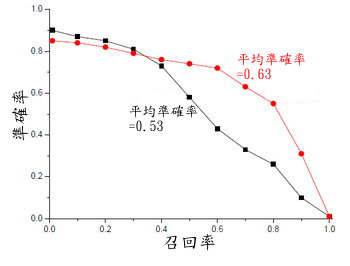
\includegraphics[scale=1.0]{images/chap2_precision_recall.png}
\caption{準確率、召回率和平均準確率之關係} \label{fig:precision_recall}
\end{figure}

\subsubsection{P@N}

通常使用者最重視的是檢索系統傳回的前幾名結果,所以就發展出了$P@N$這個評估機制。$P@N$就是只看前N個檢索結果的正確率。例如:前五個檢索結果中有一個是相關的,那$P@5$就是20\%。

$P@N$的定義如下:
\[
P@N=\frac{\text{前N個文件裡的相關文件數}}{N}
\]

\subsubsection{平均準確率~\cite{garofolo2000trec}}

因為準確率和$P@N$都需要事先決定,當查詢詞和條件不同時,很難準確地評估兩個系統的效能。因此有人提出了平均準確率(Mean Average Precision, MAP)的概念,如圖~\ref{fig:precision_recall},平均準確率就是準確率和召回率曲線下面積的平均值。平均準確率的定義如下:
\begin{equation}
MAP = \frac{1}{|Q|} \sum_Q \frac{\sum_{d \in D^R}precision(d)}{|D^R|}
\end{equation}
其中Q代表查詢詞的集合,$|Q|$為查詢詞的總數,$D^R$為和查詢詞Q相關的文件d的集合,$|D^R|$代表和查詢詞Q相關的文件數量。precision(d)代表系統檢索出文件d時的準確率。

\section{相關回饋}
相關回饋 (Relevance Feedback) 是資訊檢索的一項重要的技術~\cite{ruthven2003survey},通常可以顯著地提升系統的成果。相關回饋基本的架構如圖 ~\ref{fig:chap2_prf},使用者輸入查詢詞之後,系統會先根據查詢詞與所有文件的相關分數 $S(Q, d)$ 排序出第一次檢索結果 (First-pass Result)。然後把第一次檢索結果中部分文件標注為與查詢詞相關的正例 (Positive Example) ,部分文件標注為與查詢詞非相關的反例 (Negative Example)
,系統會再根據標注的結果重新計算查詢詞與文件的關係,把調整後的結果呈現給使用者看。
\begin{figure}
\centering
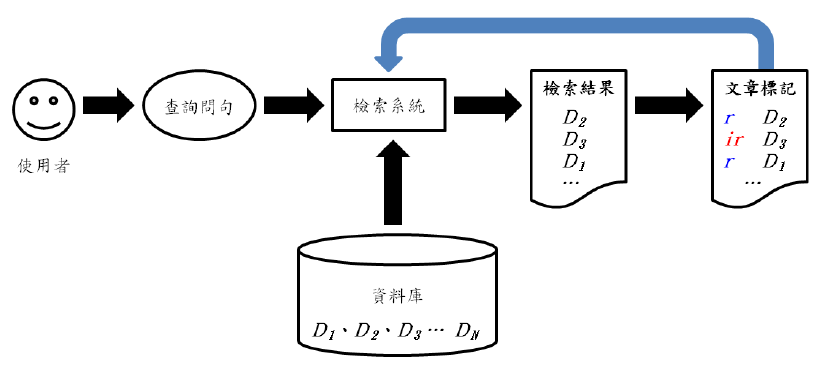
\includegraphics[scale=0.7]{images/chap2_prf.png}
\caption{相關回饋的基本架構} \label{fig:chap2_prf}
\end{figure}


把部分文件標注成正例與反例的方法可以大致分為以下幾種:

\subsection{外顯回饋}
外顯回饋 (Explicit Feedback) 的做法通常是由使用者告訴系統文件是否為正例或反例,進而增進檢索的成果。外顯回饋可分為使用者回饋 (User Feedback) 和積極回饋 (Active Feedback)
,使用者回饋是由使用者依據第一次檢索結果按照文件相關性進行標注~\cite{salton1975vector, zhai2001model, robertson1976relevance};積極回饋則是由系統主動詢問使用者某文件為正例或反例(通常是詢問系統無法決定的文件),此方法可以盡量減少使用者的標注量以改進系統的成果~\cite{tong2001support, goh2004multimodal, he2004mean}。

\subsection{隱含回饋}
隱含回饋 (Implicit Feedback) 是不由使用者直接提供正反例的資訊,而且透過觀察使用者的行為 (Behavior) 而分析文件的相關性,因此使用者並不知道自己正在回饋給系統。最常用的方法是點擊數據 (Click-through Data),比如檢索系統的前幾名如果是$d_1, d_2, d_3, ...$,而使用者沒有檢視$d_1$,而是直接檢視$d_2$,如此一來系統就可以假設$d_1$是不相關的文件,而$d_2$是相關的文件。除此之外,還可以利用查詢記錄 (Query Log)、網頁捲動
(Scrolling)和滑鼠軌跡 (Mouse Movements) 等~\cite{kelly2003implicit}。

\subsection{虛擬回饋}
虛擬回饋 (Pseudo Feedback) 不需要使用者的參與,在系統產生第一次檢索結果後,系統會直接假設其中某些部分為正例,某些部分為反例(通常是直接假設相關分數最高的$N$篇為正例,相關分數最低的$N$篇為反例)。系統會再根據這些假設進行進一步的檢索,在這個過程中,系統雖然沒有得到額外的資訊,但系統的成效通常能有一定的提升~\cite{kurland2005better, xu1996query, yu2003improving, sakai2005flexible, cao2008selecting, lee2008cluster, lv2009comparative, lv2010positional},而虛擬回饋也是此篇論文的主要研究主題之一。

\section{本章總結}
本章介紹了資訊檢索的背景,包含了基礎的資訊檢索架構、口述語彙偵測與語意檢索的差別,以及相關回饋的基本概念,並介紹了語音檢索系統的兩個主要的部分:辨識系統與檢索系統,最後介紹了動態時間扭曲做為口述語彙偵測的方法。

\chapter{以自動習得之聲學組型加強監督式語意檢索}
  \section{簡介}
傳統的語意檢索是為了檢索純文字的文件,一個很成功的解決方式是查詢詞擴展 (Query Expansion)~\cite{tao2006regularized, lavrenko2001relevance, lv2009comparative}。當系統試圖對語音文件實作查詢詞擴展時,通常的實作方法是先將語音文件辨識成文字,再對這些文字文件套用查詢詞擴展,然而這種做法的缺點是辨識過程中不可避免地會出現辨識錯誤、辭典外詞彙而導致辨識結果不準確,進而影響到檢索結果。而且許多語音文件本身帶有的語音資訊如音高、聲調等等在被辨識成文字後就消失了且再也找不回來, 過去已有許多文獻使用聲學中的資訊以幫助語音文件檢索~\cite{parada2009query, norouzian2012exploiting, lee2012open, lee2011improved, lee2012integrating},而這也是本章想探討的方向。本章中提出的解決方法使用一套自動尋找的聲學片段 (Automatically Discovered Acoustic Patterns)~\cite{lee2012nonparametric, jansen2011towards, jansen2010towards, park2008unsupervised, stouten2008discovering, wang2011iterative, vanhainen2012word, driesen2012fast, zhang2010towards} 並將語音文件辨識成這些聲學片段的序列,而這些聲學片段是直接根據輸入信號的特性去尋找的,所以可以彌補文字查詢詞擴展在語音辨識階段損失的資訊,在過去已有文獻將聲學片段應用於語音文件分類 (Spoken Document Classification)~\cite{siu2010improved, hazen2011topic, gish2009unsupervised, chaudhuri2011unsupervised}、口述語彙偵測~\cite{lee2012nonparametric, huijbregts2011unsupervised, chan2011unsupervised, wang2012acoustic}、音樂檢索~\cite{riley2008text}和影片檢索~\cite{liu2010coherent}。

查詢詞擴展是一套基於虛擬回饋的架構,當使用者輸入文字形式的查詢詞後,系統會產生第一次檢索結果,並假設前 $N$ 篇都是與查詢詞虛擬相關 (Pseudo Relevant) 的,稱為虛擬相關文件 (Pseudo Relevant Document) 再根據最大概似估計 (Maximum Likelihood Estimation) 計算出最有可能與查詢詞語意相關的詞彙加入到查詢詞中。有了每個語音文件辨識成的聲學片段序列後,根據第一次檢索結果可以得知哪些語音文件與查詢詞是虛擬相關,並假設那些常出現在虛擬相關文件中的聲學片段為與查詢詞語意相關的,再根據這些聲學片段去檢索所有的聲學片段序列得到另一份檢索結果,最後由於聲學片段成效不如文字穩定,因此將此檢索結果與文字檢索結果疊加後可得穩定進度的成效。如此一來,即使文件中包含了辭典外詞彙或是辨識錯誤,也可以從聲學片段的檢索中找出來。

\section{傳統監督式語音文件語意檢索}
\label{sec:chap4_semantic_retrieval}
語意檢索的目的是要找出所有與查詢詞語意上相關的文件,其中一種解決方式是查詢詞擴展 (Query Expansion) ,查詢詞擴展可以找出在目標文件集合中與查詢詞語意上相關的詞彙,並將其加入到原查詢詞的集合中,成為新的一組查詢詞,稱為擴展後的查詢詞 (Expanded Query) ,系統會自動使用這組新的查詢詞進行一次新的檢索,這次檢索回傳的文件就會包含擴展後的查詢詞,因此這些文件就會是與原查詢詞語意上相關的文件。

查詢詞擴展使用虛擬回饋的框架,檢索系統在使用者輸入文字形式的查詢詞後,會根據第2章的方法檢索出第一次檢索結果,再假設排序結果的前 $N$ 篇都是與查詢詞虛擬相關的文件,再利用查詢詞擴展找出這些虛擬相關文件中較常共同出現的詞彙,並將這些詞彙加入原查詢詞中,成為新的一組查詢詞,稱為擴展後查詢詞 (Expanded Query) ,系統再利用擴展後查詢詞進行下一次檢索後將結果回傳給使用者,即為傳統監督式語音文件語意檢索的做法。

查詢詞擴展的方法簡介如下:

\subsubsection{前處理}
\label{sec:preprocessing}
本章使用的檢索方式主要是基於語言模型的檢索 (Language Model Based Retrieval),因此首先要把辨識所得的詞圖轉換為語言模型。對語音文件$x$中的每個詞$t$,它在詞圖中的期望出現次數 (Expected Count) 可以如此計算:

\begin{equation}
E[t|x] = \sum_{\mu \in L(x)} N(t, \mu)P(\mu|x)
\end{equation}

$L(x)$是$x$的詞圖中所有的路徑,$\mu$是$L(x)$中的一條路徑,$N(t, \mu)$是$t$在$\mu$中出現的次數,$P(\mu|x)$是路徑$\mu$的事後機率(Posterior Probability)。

有了$E[t|x]$之後,就能把詞圖表示成單聯詞語言模型$\theta_x$:

\begin{equation}
P(t|\theta_x) = \frac{E[t|x]}{\sum_tE[t|x]}
\end{equation}

因為$\theta_x$裡沒有包含每個詞,為了讓$\theta_x$中每個詞都有一點機率,會再把$\theta_x$與一個背景語言模型 (Background Language Model) $\theta_b$做線性疊加,這個過程稱為平滑化,平滑化後的語音文件模型為$\bar{\theta}_x$。$\theta_b$可以如此估計:
\begin{equation}
\label{equ:chap3_bgm}
P(t|\theta_b) = \frac{\sum_{x\in C}E[t|x]}{\sum_t\sum_{x\in C}E[t|x]}
\end{equation}

$C$ 是所有語音文件$x$的集合。

\subsection{第一次檢索結果}
\label{sec:chap3_fpr}
查詢詞也可以被表示成語言模型$\theta_q$:
\begin{equation}
P(t|\theta_q) = \frac{N(t, q)}{|q|}
\end{equation}


$N(t, q)$ 是詞彙$t$在查詢詞$q$中出現的次數,$|q|$是查詢詞$q$中所有的詞彙總數。第一次檢索結果是由排序以下分數$S_0(q, x)$得到:

\begin{equation}
\label{equ:chap3_fpr}
S_0(q, x) = -[(1-w_1)KL(\theta_q^{w}|\bar{\theta}_x^{w}) + w_1KL(\theta_q^{s}|\bar{\theta}_x^{s})]
\end{equation}

上式同時使用了詞單位的語言模型$\theta_q^w, \bar{\theta}_x^{w}$和字單位的語言模型$\theta_q^{s}, \bar{\theta}_x^{s}$。$w_1$是線性疊加兩者時的權重。

\subsection{查詢詞擴展}
\label{sec:prf}
這裡使用正規化查詢詞混合模型 (Query-Regularized Mixture Model) 作為查詢詞擴展的實作方法,這套方法假設每篇文件都是由查詢詞相關詞彙 (Query-Related Terms) 和一般詞彙 (General Words)
所組成,而這兩者的比例在每篇文件中都是不一樣的。舉例來說,當一篇實際上不相關的文件被錯誤地假設成虛擬相關文件時,這個比例應該要很低,而反之亦然。然而實際上這個比例是不知道的,不過可以從虛擬相關文件中估計出來這個比例,估計完之後新的查詢詞模型稱為 $\theta_Q^{'}$,用來取代原本的 $\theta_Q$。

假設所有的文件為集合 $D$ 包含了文件 (已經過第一次檢索排序後) ${d_1, d_2, ..., d_n, ...}$,因此虛擬相關的文件為 ${d_1, d_2, ..., d_m, ..., d_M}$,而 $M$ 是虛擬相關文件的總數。每一篇文件中的字都可以看作是由背景語言模型 (Background Language Model) $\theta_b$ 產生,或是由新的查詢詞模型 $\theta_Q^{'}$ 產生,$\alpha_{d_m}$是$d_m$這篇文件中詞彙由 $\theta_Q^{'}$ 產生的機率,反之 $(1-\alpha_{d_m})$ 則是由背景模型 $\theta_b$ 產生的機率。透過最大概似估計最大化下式即可以估計出
$\theta_Q^{'}$ 和每一篇 $d_m$ 的 $\alpha_{d_m}$:

\begin{equation}
\label{equ:prf_f1}
F_1(\theta_Q^{'}, \alpha_{d_1}, ..., \alpha_{d_M}) = \Pi^M_{m=1} \Pi_w (\alpha_{d_m} P(w|\theta_Q^{'}) + (1 - \alpha_{d_m}) P(w|\theta_b))^{P(w|\theta_{d_m})}
\end{equation}

上式中,產生詞彙 $w$ 的機率為 $\alpha_{d_m} P(w|\theta_Q^{'}) + (1-\alpha_{d_m}) P(w|\theta_b)$ 。然而,如果只最大化式~\ref{equ:prf_f1},$\theta_Q^{'}$ 中主要會包含這些虛擬相關文件的主題,而不一定是查詢詞相關的詞彙,為了要解決這個問題,比較好的方法是用原本的查詢詞模型 $\theta_Q$ 正規化 (Regularize) $\theta_Q^{'}$,因此定義 $F_2(\theta_Q^{'})$ 如下:

\begin{equation}
\label{equ:prf_f2}
F_2(\theta_Q^{'}) = \Pi_w P(w|\theta_Q^{'})^{P(w|\theta_Q)}
\end{equation}

當 $\theta_Q^{'}$ 與 $\theta_Q$ 越近時,$F_2(\theta_Q^{'})$的值會越大。

有了式~\ref{equ:prf_f1}和式~\ref{equ:prf_f2}後,只要最大化下式即可估計 $\theta_Q^{'}$ 和 $\alpha_{d_m}$ :

\begin{equation}
\label{equ:prf_f1f2}
F_1(\theta_Q^{'}, \alpha_{d_1}, ..., \alpha_{d_M}) = F_1(\theta_Q^{'}, \alpha_{d_1}, ..., \alpha_{d_M}) F_2(\theta_Q^{'})^\lambda
\end{equation}

$\lambda$ 是個用來控制 $F_2(\theta_Q^{'})$ 影響力的參數,$\lambda$ 越大,新的查詢詞模型 $\theta_Q^{'}$ 就會跟原本的查詢詞模型 $\theta_Q$ 越像。最大化式~\ref{equ:prf_f1f2} 的好處是新的查詢詞不會過適 (Overfit) 到虛擬文件,而會保留與原本的查詢詞模型 $\theta_Q$ 一定程度的相似性。	

最大化式 ~\ref{equ:prf_f1f2} 可以採用 EM 演算法 (Estimation-Maximization Algorithm):

E step: 對於${d_1, d_2, ..., d_M}$ 中的每篇文章中的每一個詞彙 $w$:

\begin{equation}
\label{equ:prf_estep}
P(R|w, d_m) = \frac{\alpha_{d_m} P(w|\theta_Q^{'})}{\alpha_{d_m} P(w|\theta_Q^{'}) + (1-\alpha_{d_m}) P(w|\theta_b)}
\end{equation}

M step: 對於 ${d_1, d_2, ..., d_M}$ 中的每篇文章:

\begin{equation}
\label{equ:prf_mstep}
\alpha_{d_m} = \sum_w P(R|w, d_m)P(w|\theta_d)
\end{equation}

對每個詞彙 $w$:

\begin{equation}
P(w|\theta_Q^{'}) = \frac{\lambda P(w|\theta_Q)+\sum^M_{m=1} P(w|\theta_d) P(R|w, d_m)}{\lambda + \sum_w \sum^M_{m=1} P(w|\theta_d) P(R|w, d_m)}
\end{equation}

重覆地執行 E Step 和 M Step 即可得到新的查詢詞模型 $\theta_Q^{'}$

\section{以聲學片段改善監督式語意檢索}
上一節提到的傳統監督式語意檢索確實可以很好地找出與查詢詞語意上相關的文件,但由於語音文件被辨識成文字文件時很有可能會出現辨識錯誤,或某些詞彙可能是辭典外詞彙,進而使得查詢詞擴展遇到困難。事實上當系統將語音文件辨識成文字文件時,就已經損失了很多資訊,並且這些資訊是再也找不回來的了,因此這節的目的是要再利用這些聲學的資訊彌補查詢詞擴展。

本論文提出了一個系統解決以上的問題,如圖 ~\ref{fig:chap3_system}。在圖 ~\ref{fig:chap3_system}的左下角系統會自動從所有文件的集合中學出一套詞單位和字單位 的聲學片段的聲學模型和語言模型,再將語音文件用這套聲學片段辨識出來。因此圖 ~\ref{fig:chap3_system} 中的下半部將每個語音文件都表示成兩種格式:由語音辨識系統辨識而成的詞圖、由聲學片段組成的聲學片段串列。

當使用者輸入一個文字的查詢詞時,系統會將查詢詞與詞圖作比對 (圖中的右邊偏下) 並產生第一次檢索結果,系統並不會將這套第一次檢索結果回傳給使用者,而是假設其中的前
$N$篇是與查詢詞虛擬相關的,系統再利用這些虛擬相關文件作查詢詞擴展並用新的查詢詞模型檢索出一套新的檢索結果。接下來用聲學片段再做一次查詢詞擴展,即可得到聲學片段的查詢詞模型,聲學片段的查詢詞擴展假設其虛擬相關文件與文字的查詢詞擴展時相同,於是可得另一份新的查詢詞模型並用其檢索出另一套新的檢索結果,最後再把兩份檢索結果做線性疊加再排序後回傳給使用者。如此一來,即使在文字的查詢詞擴展時有些詞彙被錯誤地辨識或是有辭典外詞彙,也可以透過聲學片段的查詢詞擴展將對應到這些字的聲學片段加到聲學片段的查詢詞模型中,於是仍然可以找到包含有這些詞彙的文件。

\begin{figure}
\centering
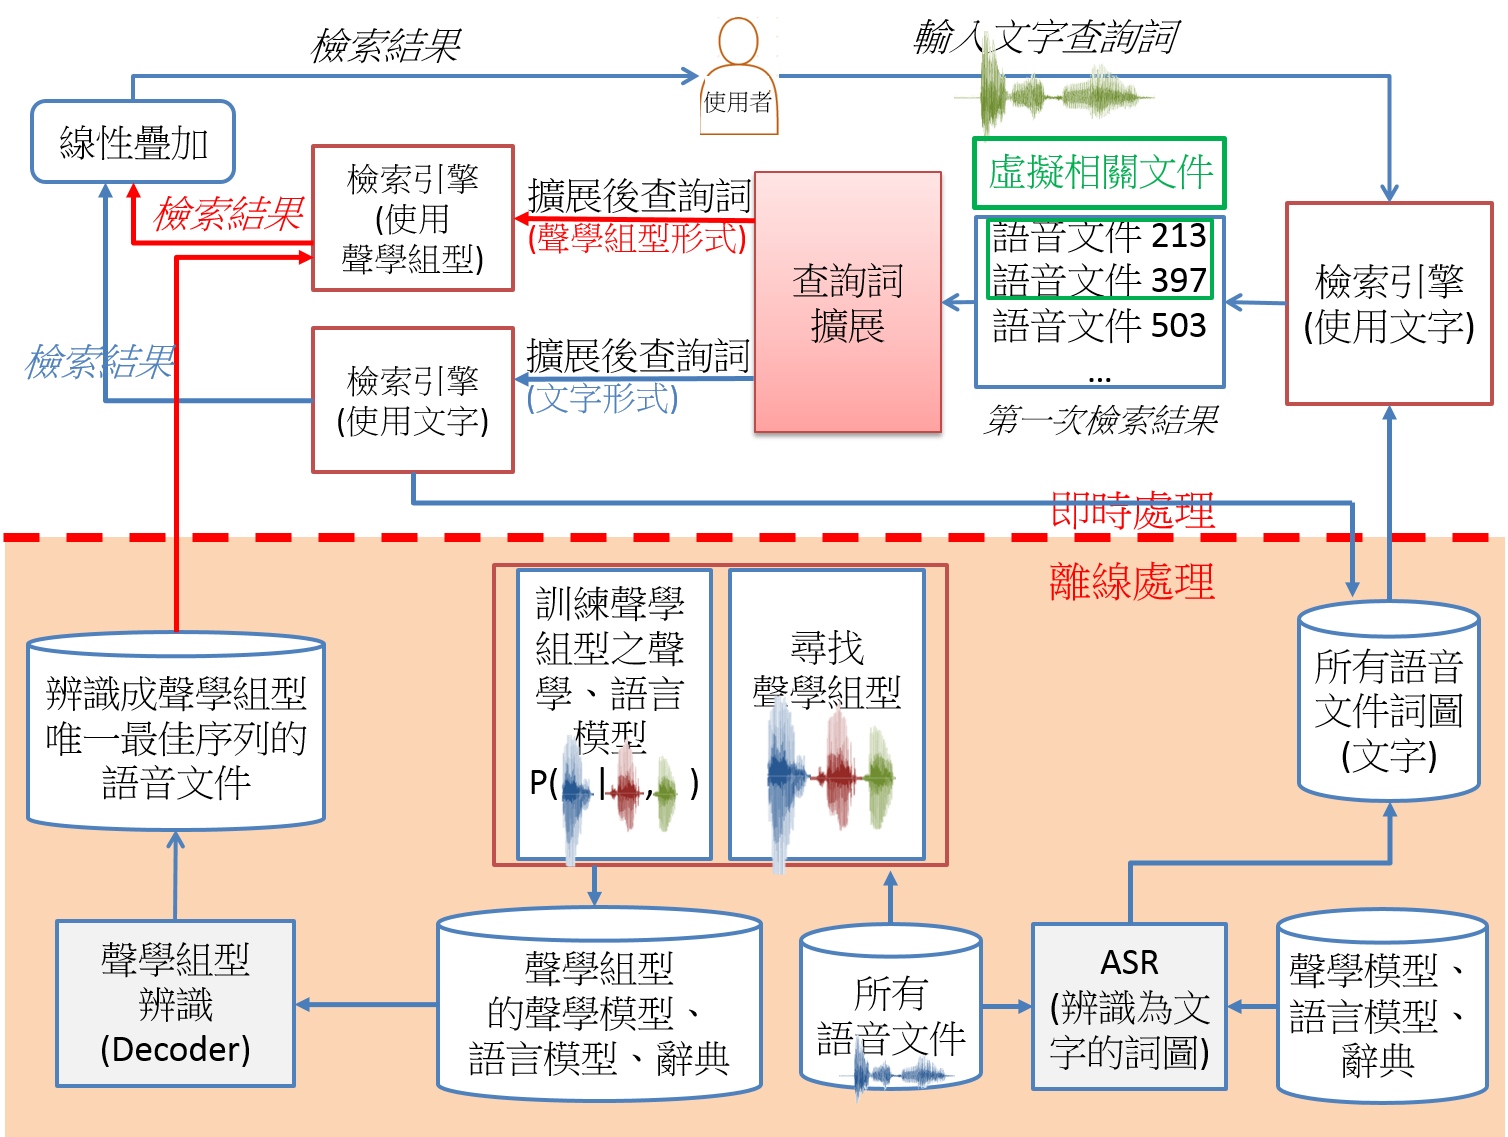
\includegraphics[scale=0.5]{images/chap3_system_zh.png}
\caption{系統架構示意圖} \label{fig:chap3_system}
\end{figure}

\subsection{前處理}
此處文字形式的前處理方式同~\ref{sec:preprocessing},即可得到由詞圖轉換而成的語音文件模型$\bar{\theta}_x$。

\subsubsection{聲學片段語言模型}
\label{sec:chap3_apd}
聲學片段指的是在某個特定語料中時常重複出現的聲音,比如像中文的音節、字等單位,這些聲學片段可以被用在口述文件分類、口述語彙偵測、語音文件檢索等。這裡使用的是本實驗室過去提出的雙層式聲學片段 (Two-Level Acoustic Pattern)~\cite{chung2013unsupervised},其中包含了約莫詞單位的聲學片段 (詞單位的聲學片段是由數個字單位的聲學片段所組成)和約莫字單位的聲學片段、字單位與詞單位聲學片段的辭典、詞單位聲學片段的N連語言模型 (N-gram Language
Model)。每個字單位聲學片段就是一個隱藏式馬可夫模型,所有的隱藏式馬可夫模型的參數、字單位聲學片段的數目、詞單位聲學片段的數目和詞單位聲學片段的N連語言模型都是在非監督式的狀況下自動地從語料庫學習出來的。學習出聲學片段以後,這些聲學模型、語言模型和辭典可以用來建立一個辨識系統,並將這些語音文件辨識成聲學片段的序列,如此即可將語音文件$x$表示成聲學片段的語言模型$\phi_x$:

\begin{equation}
P(v|\phi_x) = \frac{C(v, x)}{\sum_v C(v, x)}
\end{equation}

$C(v, x)$ 為聲學片段$v$在語音文件$x$中出現的次數。$\phi_x$會再與聲學片段背景語言模型$\phi_b$ (同式 ~\ref{equ:chap3_bgm})做平滑化(即線性疊加),平滑化的語音文件模型為$\bar{\theta}_x$。

\subsection{第一次檢索結果}
由於查詢詞$q$是文字形式的,因此第一次檢索結果只能用查詢詞模型$\theta_q$與文字的文件模型$\bar{\theta}_x$做比對,而不能使用聲學片段的文件模型$\bar{\phi}_x$
。所以計算第一次檢索結果的相關分數$S_0(q, x)$同式 ~\ref{equ:chap3_fpr}。

\subsection{查詢詞擴展}
以下簡介文字型式的查詢詞擴展與聲學片段形式的查詢詞擴展如下:

\subsubsection{文字形式的查詢詞擴展}
此處的查詢詞擴展與 ~\ref{sec:prf} 中類似,計算方法與式~\ref{equ:prf_f1f2}相似,只要最大化下式即可:

\begin{equation}
\label{equ:prf_f1f2_text}
F_1(\theta_{qe}, \alpha_{d_1}, ..., \alpha_{d_M}) = F_1(\theta_{qe}, \alpha_{d_1}, ..., \alpha_{d_M}) F_2(\theta_{qe})^\lambda
\end{equation}

$\theta_{qe}$ 即為擴展後的文字查詢詞模型,最大化上式的方法採用 EM 演算法,同式 ~\ref{equ:prf_estep} 與式 ~\ref{equ:prf_mstep}。

\subsubsection{聲學形式的查詢詞擴展}
此處的查詢詞擴展也與 ~\ref{sec:prf} 中相似,一樣是最大化下式:

\begin{equation}
\label{equ:prf_f1f2_acoustic}
F_1(\phi_{qe}, \alpha_{d_1}, ..., \alpha_{d_M}) = F_1(\phi_{qe}, \alpha_{d_1}, ..., \alpha_{d_M}) F_2(\phi_{qe})^\lambda
\end{equation}

$\phi_{qe}$ 即為擴展後的聲學片段查詢詞模型,最大化上式一樣可採用 EM 演算法,同式 ~\ref{equ:prf_estep} 與式 ~\ref{equ:prf_mstep}。

\subsubsection{線性疊加}
有了文字的查詢詞模型與聲學片段的查詢詞模型後,即可計算查詢詞$q$與文件$x$的相關分數$S(q, x)$並排序後回傳給使用者:
\begin{equation}
\label{equ:prf_interpolation}
S(q, x) = -{(1-w_2)[(1-w_1)KL(\theta_{qe}^{w}|\bar{\theta}_x^{w}) + w_1KL(\theta_{qe}^{s}|\bar{\theta}_x^{s}] + w_2KL(\phi_{qe}|\bar{\phi}_x)}
\end{equation}

% $\theta_{qe}^w$ 為詞彙的查詢詞模型,$\theta_x^w$為詞彙單位的文件模型,$\theta_{qe}^s$為次詞單位的查詢詞模型,\theta_

\section{實驗設定}
\label{sec:chap3_exp_design} 
本章的實驗使用的語料為2001年間從電台廣播中錄下的4小時新聞,並手動切成5034篇語音文件,每篇語音文件大約包含了$1至3$句的語句。用來辨識的語言模型是用1999年間收集的新聞文章 (包含4000萬個詞彙) 訓練而成,辭典中包含了62000個詞彙,聲學模型是用2000年間收集的8小時廣播新聞訓練而成的音節內(Intra-syllable) 右方資訊相依(Right-context-dependent) 聲韻母模型 (Initial-Final models)。辨識後的唯一最佳序列的字元正確率為 (Character Accuracy) 為75.27\%。
總共測試了29組查詢詞,每組查詢詞都有人工標注對應的語意相關文件,而這些語意相關文件中「並不一定要」包含查詢詞。本章中使用平均準確率做為評量標準。

\section{實驗結果及分析}

圖 ~\ref{fig:chap3_resulta} 中顯示的是式 ~\ref{equ:prf_interpolation} 疊加的結果,其中 $\lambda$ 固定為 800,$N$ 為 $5, 10, 15, 20, 25$ ,紅線則是第一次檢索結果,是不使用查詢詞擴展時的結果。縱軸是平均準確率(MAP),橫軸則是式 ~\ref{equ:prf_interpolation} 的$w_2$,為聲學片段與文字的擴展後查詢詞疊加時的權重,$w_1$在實驗中都被固定為 $0.95$。首先來比較第一次檢索結果與文字的查詢詞擴展後的結果 $(w_2 =
0)$時的狀況,可以觀察到文字的查詢詞擴展比第一次檢索結果好上一些,即使它可能有受到辨識錯誤或辭典外詞彙的影響。接下來看有使用聲學片段時的狀況:當 $w_2$大於零時,可以注意到整體的平均準確率相對 $w_2 = 0$時都是進步的 (只要$w_2 < 0.5$),這代表了使用聲學片段確實能夠幫助查詢詞擴展找到更多聲學方面的資訊,進而使平均準確率更為進步。另一方面也可以看到,當 N 增加,平均準確率會先成長後再下降,大約在 $N=10$
的時候為最佳的狀況,這個原因是由於當$N$變多時,被假設為虛擬相關的文件數也變多,因此更多的資訊被用來進行虛擬回饋,但另一方面如果假設了太多的虛擬文件時,會使用太多不相關資訊進行虛擬回饋,使得系統的平均準確率下降,最好的平均準確率是在 $N=10$而且 $w_2 = 0.40$ 的狀況,而這代表說文字的查詢詞擴展是比聲學片段的查詢詞擴展來得可靠的,因此文字查詢詞擴展的權重必須要設得高一些,由於這是最好的結果,所以在之後的實驗中會將 $N$ 設為 10。

圖 ~\ref{fig:chap3_resultb} 和圖 ~\ref{fig:chap3_resulta} 類似,只是圖 ~\ref{fig:chap3_resultb} 中將 $N$ 固定為 10,並且測試不同的 $\lambda$,在圖中可以發現當 $\lambda$ 很低的時候 (如100),系統的平均準確率甚至是比第一次檢索結果還要差的,然而當 $\lambda$ 夠大的話 ($\lambda \geq 400$),系統的平均準確率都是比第一次檢索結果和 $w_2 = 0$ 的狀況還要好的。這證明了式 ~\ref{equ:prf_f2} 的重要性,如果 $\lambda$ 太小的話就會導致系統在訓練時對於虛擬文件過適而使得成果更差,而 $\lambda$ 夠大時 ($\lambda > 400$) 就幾乎都能看到不錯的進步 。  

\begin{figure}
\centering
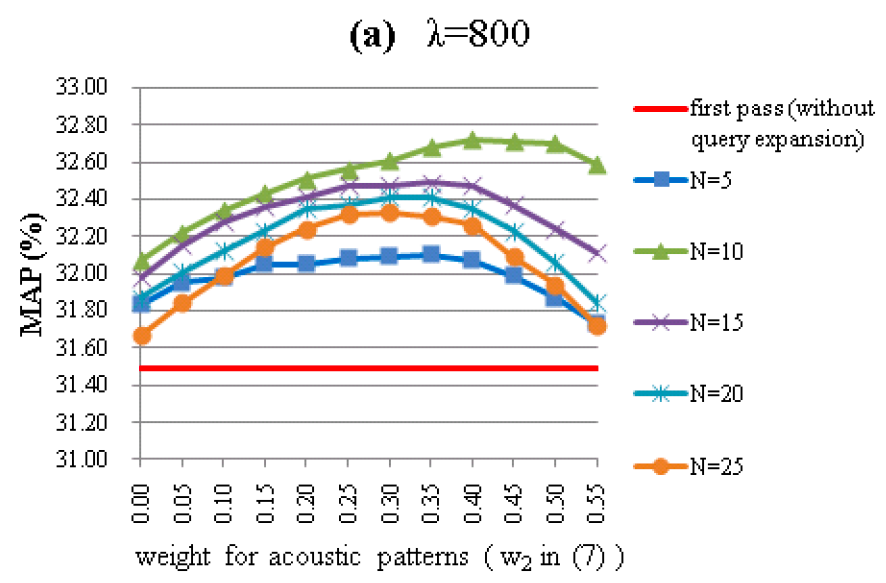
\includegraphics[scale=0.4]{images/chap3_resulta.png}
\caption{將文字形式和聲學片段形式的查詢詞擴展疊加後的平均準確率 ($\lambda = 800$)} \label{fig:chap3_resulta}
\end{figure}

\begin{figure}
\centering
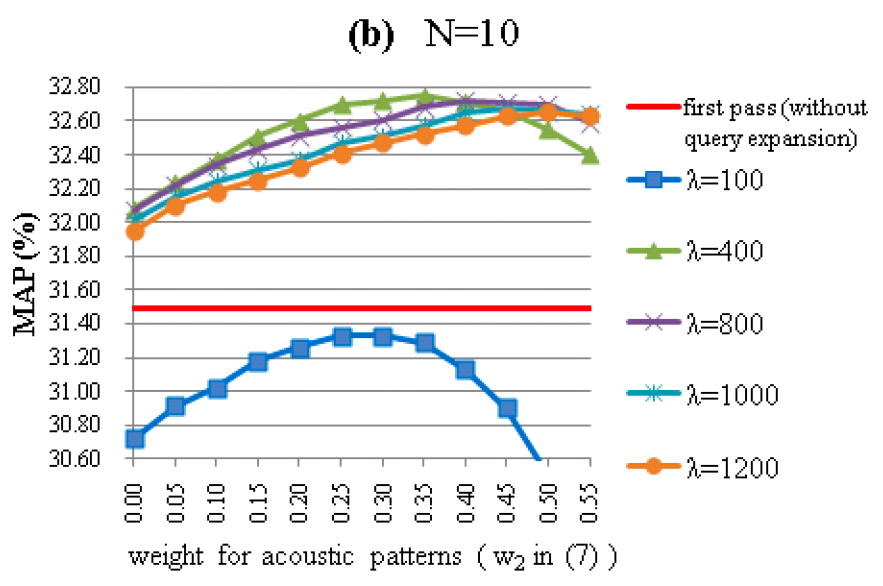
\includegraphics[scale=0.4]{images/chap3_resultb.png}
\caption{將文字形式和聲學片段形式的查詢詞擴展疊加後的平均準確率 ($N=10$)} \label{fig:chap3_resultb}
\end{figure}

圖 ~\ref{fig:chap3_resulta} 和圖 ~\ref{fig:chap3_resultb} 中表示了將文字形式和聲學片段形式的查詢詞擴展疊加後的平均準確率,縱軸為平均準確率(MAP),橫軸為線性疊加中聲學片段的權重。圖中的紅色橫線是第一次檢索結果的平均準確率 (不含查詢詞擴展)。

\section{本章總結}
在本章中使用了聲學片段加強監督式語音文件語意搜索的成效,如此一來可以解決諸如辨識錯誤、語音文件中包含詞典外詞彙的問題,可以有效提升語意檢索的平均準確率。


\chapter{以自動習得之聲學組型實現非監督式語意檢索}
  \section{簡介}

\section{使用動態時間扭曲之無監督式文件搜尋}

\section{基於語音片段之語義搜尋}

\section{實驗基礎架構}

\section{實驗設計}

\section{實驗結果及分析}

\section{本章總結}

\chapter{利用遞迴式類神經網路語言模型加強非監督式語音文件檢索}
  \section{簡介}

\section{基於遞迴式類神經網路語言模型之詞向量}

\section{以詞向量改善無監督式語義搜尋}

\section{實驗基礎架構}

\section{實驗結果}

\section{實驗結果及分析}

\section{本章總結}

\chapter{在Google Glass上實作個人化的語音翻譯與新聞檢索系統}
  \section{簡介}
隨著近年來行動裝置與雲端運算的興起,行動裝置逐漸成為了業界的兵家必爭之地,許多公司都喊出了「行動優先」口號,足見業界對於行動裝置平台之重視,如Google、Facebook、Apple等科技大廠皆紛紛搶入行動裝置平台。由於行動裝置小、鍵盤輸入介面不方便、往往需要在移動時輸入等特性,使得語音輸入在行動裝置上相形重要,因為語音相對於傳統的鍵盤輸入是更自然也更貼近人性的輸入方法。但行動裝置上的語音輸入不比傳統的語音輸入,有許多與傳統語音輸入不同的特性,由於這些特性將導致一些困難的挑戰和更多有趣的性質可供研究,以下將簡介這些特性。

第一個特性為自發性語音 (Spontaneous) 含發音差異 (Pronounciation Variation)、不流暢性 (Disfluency)、語速變化 (Speaking Rate Variation)~\cite{DBLP:conf/interspeech/YehLL13}及背景雜訊 (Background Noise),由於使用者使用行動裝置上的語音輸入時往往是很自發性地 (Spontaneous) 說話,因此這些語速是很不固定的,將隨著使用者的使用情景、當下的情緒等等而改變,另一方面行動輸入通常會在有背景雜音的狀況下輸入,如馬路上、百貨公司中,會附有很多的背景雜音,因此語速變化與背景雜音可以說是行動語音輸入最主要的困難之一。

第二個特性為個人化 (Personalization),這是由於行動裝置通常只屬於某一特定的使用者,因此行動裝置可以搜集大量的個人資訊對使用者進行個人化,使得使用者的語音辨識結果最接近他有可能說出的話。這其中包含了語音模型、語言模型與辭典的個人化~\cite{DBLP:conf/interspeech/WenHLTL13, wen2012personalized, bellegarda2004statistical},語音模型可以調適 (Adaptation) 至接近使用者語音特性的語音模型,語言模型與辭典則可以藉由收集使用者常說與常用的詞
(可以從過去的語音輸入中收集,或是從社群網路如 Facebook、Twitter上收集)進行調適。如此一來即可以將使用者的行動語音輸入個人化成最適合使用者使用的行動語音輸入。

第三個特性為行動裝置上的感測器 (Sensor),這是行動裝置上特有的特性,由於行動裝置上通常帶有全球定位系統 (Global Positioning System, GPS)
,而未來甚至可能帶有個人身體狀況的感測器,如血壓、心跳等,而這些感測器的特徵正好可用來幫助語音辨識,如裝置知道使用者的位置,就可以將當地景點、餐廳在語言模型中的機率增加,如裝置知道使用者血壓、心跳增高,可能代表使用者處於憤怒狀態,此時憤怒的詞彙在語言模型中的機率也可以被適當地增加。因此如果可以擅用這些感測器的結果,將能很好地幫助語音辨識。

本章中的個人化語音系統的應用皆實作於 Google 推出的 Google 眼鏡 (Google Glass) 之上 (如圖~\ref{fig:glass}),Google 眼鏡主體為其右上角之藍色部分,其前面包含了一塊透明的顯示器,Google 眼鏡會將顯示畫面投影到透明的顯示器上讓使用者閱讀,藍色的部分還包含了麥克風、喇叭、相機、觸控板(可偵測多種手勢)等裝置。

\begin{figure}
\centering
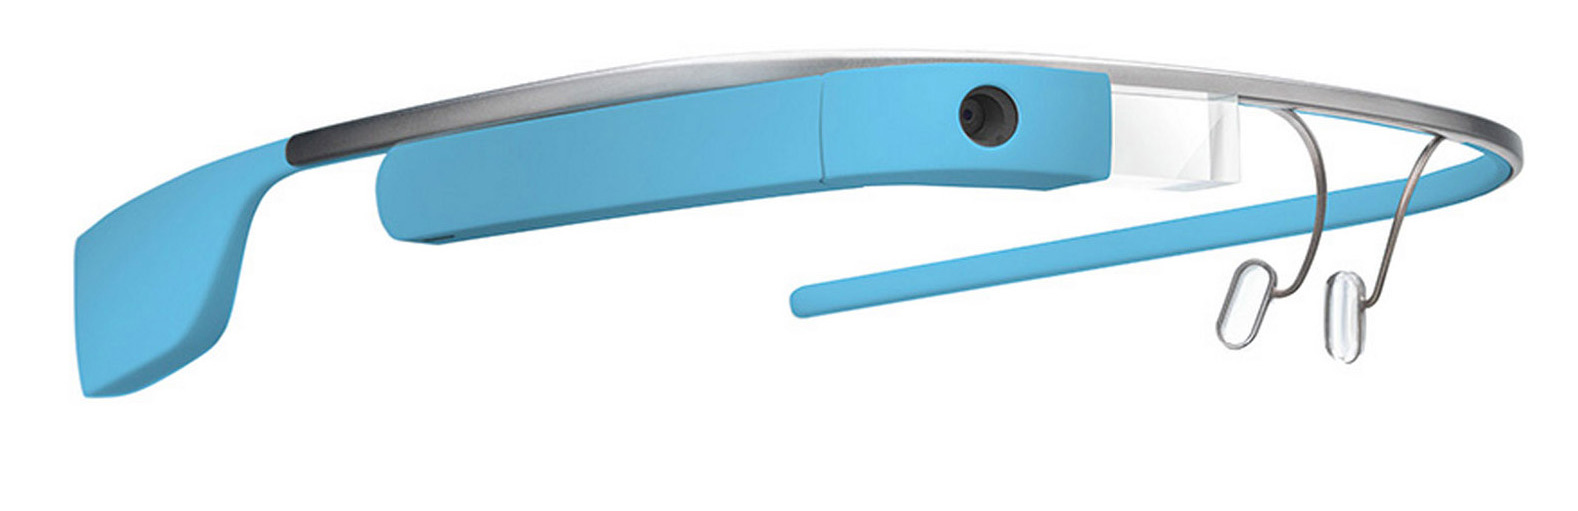
\includegraphics[scale=0.2]{images/glass.jpg}
\caption{Google 眼鏡} \label{fig:glass}
\end{figure}

\section{個人化的語言翻譯系統簡介}

以下將介紹本實驗室開發的個人化語言翻譯系統,其開發動機是由於穿戴型裝置日益流行,如果能讓使用者在旅遊或是與外國人對話的期間,一旦有不會講的話就能直接用自己的母語對裝置說話,並由裝置進行辨識與翻譯後告訴使用者該如何用另一個語言講這段話。

因此我們設計了一套個人化語言翻譯系統,利用智慧型行動裝置如手機、甚至是近年來逐漸受到重視的智慧型穿載裝置,像Google眼鏡等,讓使用者能隨時隨地地進行為自己量身打造的體驗:使用者以自己的母語講出想學的內容,行動裝置會將訊號送至雲端的個人化語音辨識系統,將語音辨識成文字,再將辨識後的文字送至Google提供的翻譯服務將文字翻譯成使用者想學的目標語言,再回傳到行動裝置讓使用者同時看到翻譯後的文字與聽見範例發音,系統示意如圖 ~\ref{fig:chap6_translation_system}

\begin{figure}
\centering
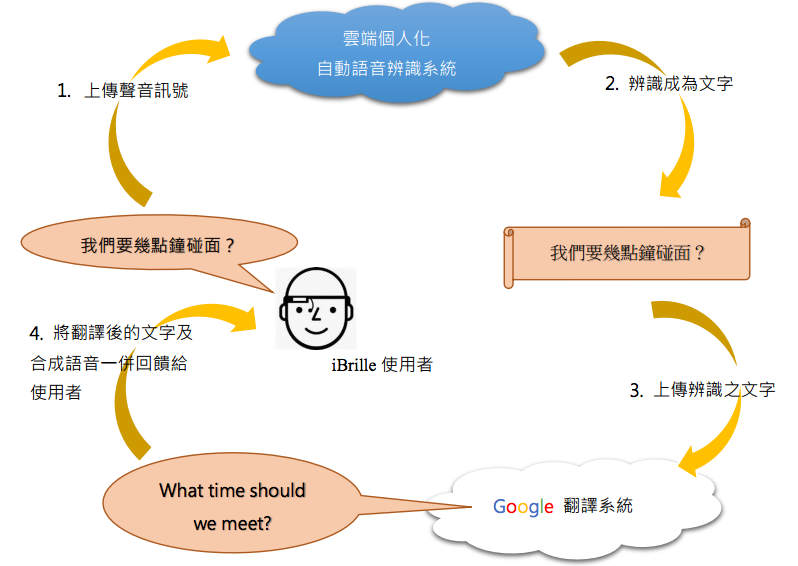
\includegraphics[scale=0.4]{images/chap6_translation_system.png}
\caption{雲端個人化語言翻譯系統架構} \label{fig:chap6_translation_system}
\end{figure}

本系統可分為兩部分:

\subsubsection{個人化自動語音辨識系統 (Personalized Automatic Speech Recognition System)} 
目前使用的雲端辨識系統可分為幾個區塊,包含聲學模型、語言模型、詞典,依序介紹如下:

\begin{itemize}

   \item 聲學模型:

聲學模型架構使用的是三連音(Triphone)隱藏式馬可夫模型(Hidden Markov Model, HMM),每一個馬可夫模態(HMM State)則是由深層類神經網路(Deep Neural Networ)的輸出層中的一個神經元(Neuron)來表示,也就是近年流行的上下文相關深層類神經網路隱藏式馬可夫模型 (Context-dependent Deep Neural Network Hidden Markov Model,
CD-DNN-HMM)。類神經網路端所輸入的語音特徵則是疊加了九個音框長度的梅爾濾波器組特徵(Mel-Filter Bank Features),維度是621維。網路中共有四層隱藏層(Hidden Layer),每一層中有2048個隱藏神經元(Hidden Neuron),輸出層則是有6647個節點。用來訓練聲學模型的語料則是結合了雙語料,其中聲碩麥克風(ASTMIC)做為中文語料以及台灣區英語(English Across Taiwan)當中非母語語者(Non-native Speaker)部分做為英文語料。
兩個語料都是收集自台灣區語者的錄音,並且都是多語者(Multi-speaker)語料,且性別各半均衡。

   \item 語言模型:

語言模型採用傳統的N連詞(N-gram)模型,並且為三連詞模型。訓練語料包含了Yahoo! 新聞(Yahoo! News)、 Gigaword、公視新聞 (PTV),並且在訓練完成後,與以聲碩麥克風與台灣區英語的訓練集語料訓練的語言模型作內插調適。

   \item 詞典:

此系統詞典中文部分包含所有常見中文單字,以及經由PAT-Tree所產生的
字詞。英文部分,則是包含卡內基美儂大學所公開之英文辭典當中,詞頻較高者。所有字詞的發音皆是音素(Phoneme)序列,包含中英雙語的所有音素。

\end{itemize}

\subsubsection{翻譯系統}

經辨識所得之文字,將送至 Google 的雲端翻譯系統,並由 Google 翻譯將其翻譯為使用者想學的目標語言,再將翻譯後的文字與合成發音一併傳回    Google 眼鏡上,將使用者想翻譯的語言呈現於屏幕上,並同步撥放發音以助翻譯。此一部分由於本實驗室尚未有完善的翻譯系統,不過一旦未來研發出辨識系統後,即可將 Google 翻譯系統替換為本實驗室自行開發之翻譯系統。

\section{個人化的語音文件檢索系統簡介}
以下將介紹本實驗室自行開發的個人化行動語音文件檢索系統,其開發動機為使用者在行動時也往往有搜尋資訊的需求,而在移動時使用鍵盤輸入對於使用者又極度地不方便,因此我們就決定開發了這套基於 Google 眼鏡的語音文件檢索系統,讓使用者能夠隨時隨地取得自己想要的資訊,使用情境如下:使用者對 Google 眼鏡輸入語音查詢詞,然後 Google 眼鏡再將訊號上傳到個人化語音辨識系統,辨識為文字後,系統再將文字的語音查詢詞上傳至
~\ref{sec:chap4_semantic_retrieval} 中提到的監督式語意文件檢索系統。檢索系統會再將檢索後的內容傳回給使用者,並呈現於 Google 眼鏡上供使用者閱讀。

本系統可分為兩部分:

\subsubsection{個人化自動語音辨識系統}

此部分同上一節個人化的語言翻譯系統中的個人化語音辨識系統。

\subsubsection{監督式語意檢索系統}

此處使用之系統同~\ref{sec:chap4_semantic_retrieval},使用的語料為2001年間從電台廣播中錄下的4小時新聞,並手動切成5034篇語音文件,每篇語音文件大約包含了1至3句的語句。用來辨識的語言模型是用1999年間收集的新聞文章 (包含4000萬個詞彙) 訓練而成,辭典中包含了62000個詞彙,聲學模型是用2000年間收集的8小時廣播新聞訓練而成的音節內(Intra-syllable)
右方資訊相依(Right-context-dependent) 聲韻母模型 (Initial-Final models)。辨識後的唯一最佳序列的字元正確率為 (Character Accuracy) 為75.27\%。
\section{系統展示}
此節將展示本系統之部分截圖與使用示例。

\subsection{個人化的語音翻譯系統展示}
本實驗室開發的個人化語音翻譯系統的名稱取為iBrille,取Brille在德語中為眼鏡,在西班牙語及法語中有閃耀的意思。圖 ~\ref{fig:ibrille_enter} 中為 iBrille 系統的首頁,一進入系統後會顯示「觀迎來到 iBrille 教學系統」,圖 ~\ref{fig:ibrille_example} 中則為使用者對 iBrille 講出一段欲翻譯的話後,由個人化的語音翻譯系統辨識、並翻譯後顯示的畫面。
\begin{figure}
\centering

\includegraphics[scale=0.3]{images/glass/ibrille_enter.png}
\caption{iBrille 首頁} \label{fig:ibrille_enter}
\centering

\includegraphics[scale=0.3]{images/glass/ibrille_example.png}
\caption{iBrille 使用示範} \label{fig:ibrille_example}
\end{figure}

\subsection{個人化的語音文件檢索系統展示}
本實驗室開發的個人化語音文件檢索系統的名稱取為「新聞隨手查」,希望能讓使用者無論在隨時隨地都能很方便迅速地吸收到感興趣的資訊。圖 ~\ref{fig:news_enter} 為新聞隨手查的首頁,而圖 ~\ref{fig:news_example} 則為使用者說出「颱風」這個查詢詞後顯示的畫面。
\begin{figure}
\centering

\includegraphics[scale=0.3]{images/glass/news_enter.png}
\caption{新聞隨手查首頁} \label{fig:news_enter}
\centering

\includegraphics[scale=0.3]{images/glass/news_example.png}
\caption{新聞隨手查使用示範} \label{fig:news_example}
\end{figure}

\section{本章總結}
行動裝置在這幾年內漸形重要,因此也使得在行動裝置上的語言輸入漸受重視,本章中利用了 Google 眼鏡實作了個人化的語音翻譯系統與個人化的語音文件檢索系統,將個人化的語音辨識系統與行動裝置上的應用程序結合起來,成為對使用者更為方便的應用程序。

\chapter{結論與展望}
  \section{本論文主要的研究貢獻與未來展望}
\subsection{使用聲學組型加強語音文件檢索}
本論文中主要貢獻在於利用聲學組型解決傳統語音檢索的難題,由於傳統的語音文件檢索是先辨識後在詞圖上檢索,但有許多聲學上的資訊在辨識之後就消失了,因此本論文試圖在檢索時加入聲學組型的資訊以提升檢索系統成效,主要貢獻條列如下:

1. 使用聲學組型加強監督式語音文件的語意檢索系統,因為傳統的語音文件檢索是先辨識後在詞圖上檢索,但如果此時有辭典外詞彙或是辨識錯誤的話,檢索結果就會很差了,因此本論文使用聲學組型解決此難題。

2. 使用聲學組型達成非監督式語音文件的語意檢索系統,傳統的語意檢索系統需要先將語音文件辨識成詞圖後才進行語意檢索,但是這樣需要已訓練得很好的聲學模型和語言模型,而這兩者的訓練通常是非常昂貴的,因此我們使用聲學組型解決這個問題。

3. 使用聲學組型雖然能加強以上兩種狀況,但是聲學組型有一個缺點:聲學組型在訓練時並不知道聲音和字之間的關聯,因此會將所有音同字不同的聲音都歸類到同一個聲學組型中,但如此一來在檢索時便無法區別不同的字義了,進而導致檢索的成效很差,所以我們試圖用遞迴式類神經網路語言模型產生的詞表示法來區分出同一個聲學組型中對應到不同字義的聲學組型。

\subsubsection{未來的改進方向}
由於使用聲學組型進行完全非監督式的語音文件檢索是一個十分新穎的研究題目,因此目前系統的平均準確率距離監督式語音文件檢索尚有一段距離,需要更進一步地研究,而可能的研究方向如下:

1. 將同音的聲學組型盡可能按照它對應到的字區分開來:由於目前的聲學組型是將同音的組型盡量分在一起,但這在檢索時會造成困難,因此如果能將聲學組型按照它對應到的字區分開來的話,將能使檢索的效能進步許多,第~\ref{sec:chap5}章 中嘗試了一些做法,但還可以嘗試不同的分群演算法和更好的詞表示法。

2. 使用詞表示法改進檢索系統:目前的檢索系統仍然是使用傳統的詞表示法,因此無法得知詞與詞之間的相似關係,如果能將檢索系統的詞表示法改為 第~\ref{sec:chap5}章中的方法,應能在語意檢索上再進步許多。

\subsection{實作雲端語音辨識與應用程式於 Google 眼鏡}
行動裝置在這幾年間快速地崛起,連帶使得行動裝置上最自然的輸入方式-語音輸入受到許多人的重視,另一方面,行動裝置上的語音辨識系統會遭遇到許多與傳統語音辨識系統不同的挑戰與機會,諸如語速的變化、聲學/語言模型/辭典的個人化、行動裝置上的感測器等等。本論文將本實驗室開發的雲端個人化語音辨識系統實作於目前最流行的穿戴式裝置-Google 眼鏡之上,並於其上建立了兩個應用程序:

1. 雲端個人化語言學習系統:使用雲端語音辨識加上Google翻譯,使學生能夠隨時隨地學習自己需要的內容。

2. 雲端個人化新聞查詢系統:使用雲端語音辨識加上~\ref{sec:chap4_semantic_retrieval}中提到的監督式語意檢索系統,讓使用者隨時隨地都能查詢自己感興趣的新聞。


%
% this file is encoded in utf-8
% v2.0 (Apr. 5, 2009)

%%% 參考文獻
\newpage
\phantomsection % for hyperref to register this
\addcontentsline{toc}{chapter}{\nameRef}
\renewcommand{\bibname}{\protect\makebox[5cm][s]{\nameRef}}
%  \makebox{} is fragile; need protect
\bibliographystyle{IEEEbib}  % 使用 IEEE Trans 期刊格式
\bibliography{thesis_bib}


%%% 附錄
%\input{my_appendix.tex}

%%% 自傳
%\newpage
%\chapter*{\protect\makebox[5cm][s]{\nameVita}} % \makebox{} is fragile; need protect
%\phantomsection % for hyperref to register this
%\addcontentsline{toc}{chapter}{\nameVita}
%\input{my_vita.tex}



\clearpage % to make sure all CJK characters are processed
\end{CJK}  %%% ZZZ %%%
\end{document} 
 
